    
\section{Exploratory Analysis}


    \subsection{Main effect subgroups}

    There are three main effects by which breast cancer samples can be stratified into groups: morphology, stage and PAM50 molecular profile. PCA is able separate samples into tumour/normal sample clusters fairly well (shown as an example in Methods, Figure \ref{fig:pcamethod}). However, it is more interesting to apply PCA to explore variation between groups of samples captured by applying different classification methods.  
    PCA was applied to 969 samples (857T, 112N), which were divided into subgroups by three systematic effect groups (i.e. PAM50, tumour morphology, cancer stage), the sizes of which are shown in Tables \ref{table:morphstage} and \ref{table:pam50counts}. \\
    The PCA plot of data coloured by PAM50 molecular subtypes is shown in Figure \ref{fig:pcapam50}. PC1 accounts for 11\% of the total variation in the data, and is driven by the differences between normal and cancer samples. PC2 accounts for 8.6\% of the variation, and characterises the variation among breast cancer subtypes. Basal-like samples form a separate cluster (orange), which emphasises its complete dissimilarity at molecular level. Luminal A and Luminal B form a partially overlapping cluster (yellow and red), which is expected from the known similarities of these subtypes. HER2-enriched cluster (blue) is understandably located between Luminal B and Basal-like as it is known to share expression profiles and receptor statuses with these two. And lastly, seeing Normal-like subtype (pink) overlapping with normal samples (green) as well as with Luminal A subtype fits nicely with the fact that Normal-like subtype shares morphology with the former and IHC and molecular profile with the latter.    
    
    % PAM50 PCA plot 
            \begin{figure}[!h]
            \centering
            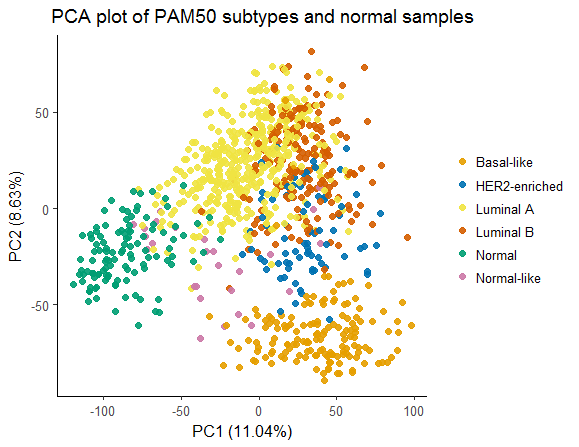
\includegraphics[scale=0.4]{pcapam502.png} 
            \caption[PCA plot showing separation by PAM50 subtypes(2D)]{PCA plot showing the variance along PC1 and PC2 for PAM50 molecular subtypes of breast cancer and normal samples.}
            \label{fig:pcapam50}
            \end{figure}
            
    \newpage
    One dimensional PCA plot based on PAM50 subtypes is shown in Figure \ref{fig:1dpcapam50}, where the variation along the first nine PCs is displayed as explained in the Methods section 2.2.1. Looking at the results in this way highlights again that PC1 is driven by tumour/normal variation. Together with PC2 they also capture the differences among PAM50 subtypes. As the PCs numbers increase, variation captured by them decreases. 
    
    % PAM50 1d PCA plot 
            \begin{figure}[!h]
            \centering
            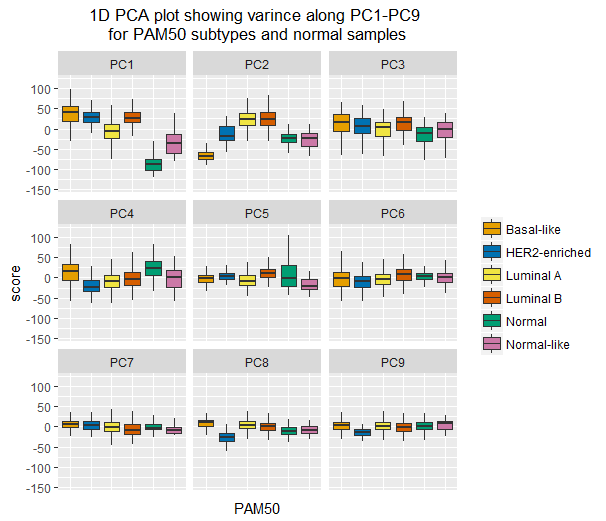
\includegraphics[scale=0.39]{1dpcapam50.png}
            \caption[PCA plot showing separation by PAM50 subtypes (1D)]{One-dimensional PCA plots showing variance along PC1-PC9 for PAM50 molecular subtypes of breast cancer and normal samples. }
            \label{fig:1dpcapam50}
            \end{figure}
    
    
    The PCA results for stages and morphology classifications are shown in Figures \ref{fig:1dpcastage} and \ref{fig:1dpcamorph} (2D ad 1D). PCA was not able to capture as much variation between morphology groups and stages as between PAM50 subtypes. From one-dimensional plots for both stages and morphology it is evident that PC1 captures cancer/normal differences in both classification types. However, the rest of PCs do not capture enough variation to be evident on 2D PCA plots. The 2D scatter plots are displaying PCs with the most prominent variation.     
    
    % 1D PCA for stages and morphology
            
            \begin{figure}[!h]
            \hspace*{\fill}
            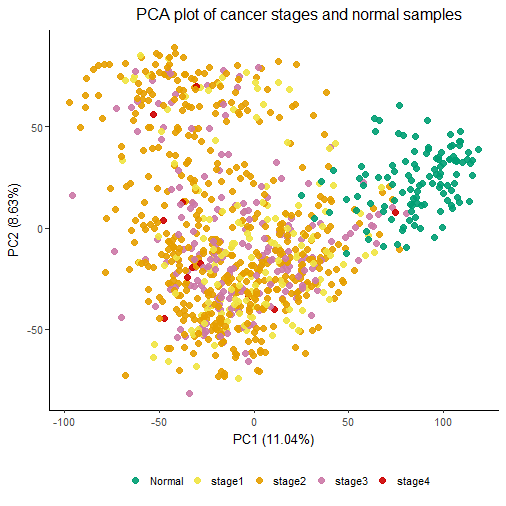
\includegraphics[width=0.51\linewidth]{pcastages.png}\hfill
            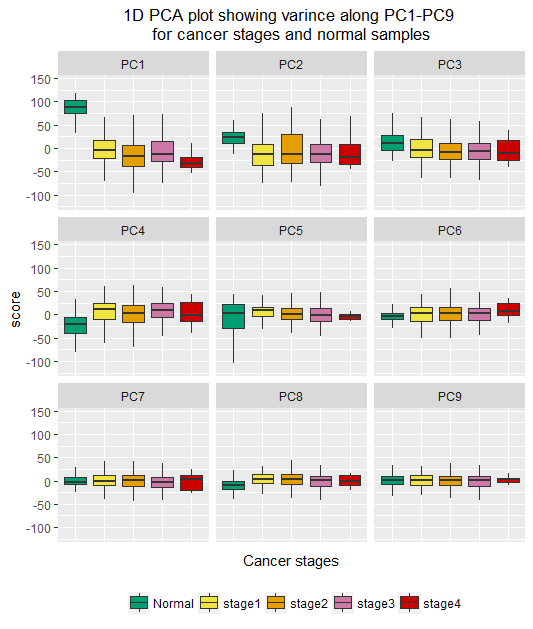
\includegraphics[width=0.44\linewidth]{1dpcastages2.png}
            \hspace*{\fill}
            \caption[PCA plots (2D and 1D) showing separation by cancer stages]{2D and 1D (PCs 1-9) PCA plots showing variance captured between cancer stages and normal samples.}
            \label{fig:1dpcastage}
            \end{figure}
            
        Interestingly, PCA did not capture any noticeable differences even between distant stages (i.e. stage 1 and stage 4), where the differences in expression should be evident and therefore reflected in PCA results. This is also the case for two main distinct morphologies - Lobular and Ductal carcinomas, which overlap greatly.
    
            \begin{figure}[!h]
            \centering
            \hspace*{\fill}
            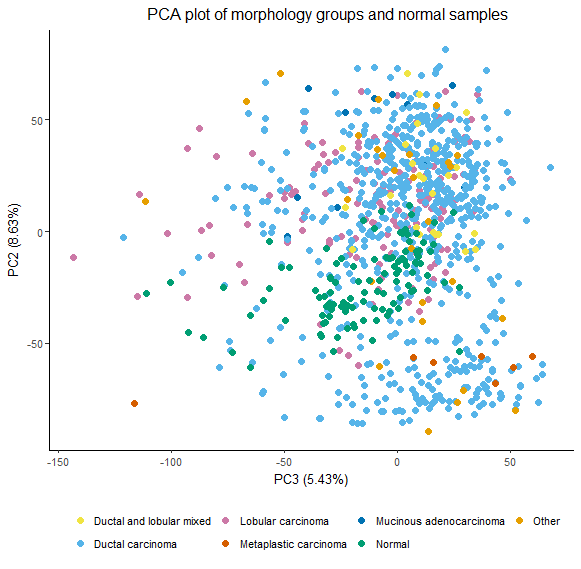
\includegraphics[width=0.48\linewidth]{pcamorph.png}\hfill
            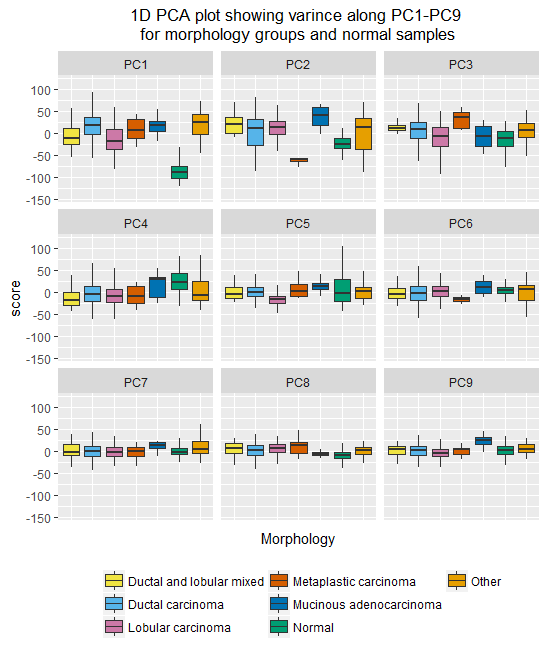
\includegraphics[width=0.41\linewidth]{1dpcamorph2.png}
            \hspace*{\fill}
            \caption[PCA plots (2D and 1D) showing separation by tumour morphologies]{2D and 1D (PCs 1-9) PCA plots showing variance captured between tumour morphologies and normal samples.}
            \label{fig:1dpcamorph}
            \end{figure}

    
    \newpage
    A possible explanation for the observed PCA results is the difference in sizes of morphology and stages subgroups, as well as their composition in terms of PAM50 subtypes, which is evidently the main driving force behind sample classifications. To explore this idea, the sample count per subgroup was visualised as stacked barplots presented in Figure \ref{fig:barms}. Each bar shows the total number of samples of a chosen morphology (left plot) or stage (right plot). The difference in groups sizes in apparent.
    % barsplots for stages and morphology 
       
        \begin{figure}[!h]
        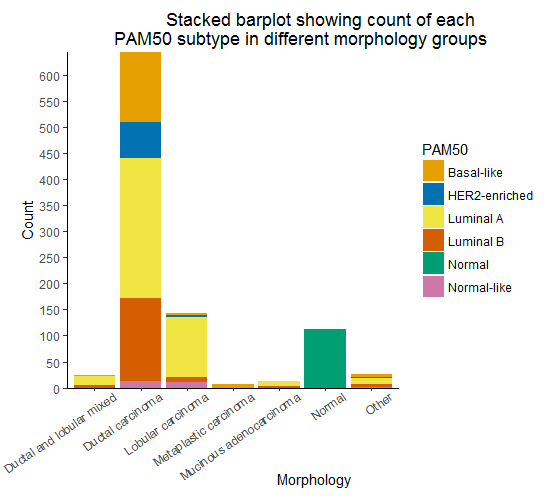
\includegraphics[width=0.53\linewidth]{bar_morph.png}\hfill
        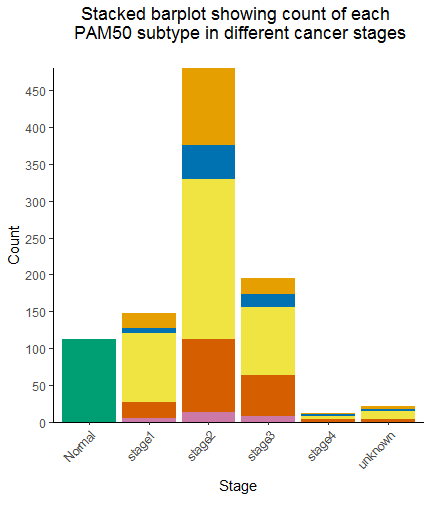
\includegraphics[width=0.4\linewidth]{bar_stages2.png}
        \caption[Stacked barplots of samples count per stage and morphology type]{Stacked barplots of sample counts per subgroups in morphology types (left) and stages (right). The coloured proportions represent PAM50 subtypes samples within each subgroup.}
        \label{fig:barms}
        \end{figure}
        
    Ductal carcinoma samples make up 75\% of all samples (644/857), but are well-proportionate in terms of their PAM50 composition (i.e. similar proportions as the full dataset, with Luminal A dominating). Other morphologies, however, in addition to being smaller in sample count, are restricted to only a few PAM50 subtypes. For instance, Metaplastic carcinoma is made up completely of Basal-like samples, while Mucinous morphology is represented by only Luminal subtypes (the counts are shown in Table \ref{table:counts}). This explains why these two mophologies are separated in 2D PCA plot in PC2 (Figure \ref{fig:1dpcamorph}) - the difference between Luminal and Basal tissues is driving their variation. However, it is important to note, that there is some evidence in the literature, a study by Weigelt \textit{et al.} \cite{Weigelt2010a} that these two morphologies, Metaplastic and Mucinous, actually only exists as Basal and Luminal subtype, so the observed difference might be truly due to morphology.  
    
    The sample count difference between stages is also noticeable, which stage 2 accounting for roughly 50\% of the samples. The proportions of PAM50 subtypes within stages 1-3 appear to be well-balanced. However, this is not the case for stage 4, where in addition to alarmingly low sample count, Normal-like subtype is not represented. The counts are shown in Table \ref{table:counts}.  \\
        
        
    %TABLE x3 counts   
                \begin{table}[!h]
                \centering
                \tiny
                \caption[Sample counts per each pairwise subgroup in the dataset]{Samples number counts in pairwise comparisons of three main breast cancer samples classifications. \textit{Top table:} PAM50 and stages,\textit{ Middle table:} PAM50 and morphology, \textit{Bottom table:} stages and morphology. Each table shows row and column sums for each subgroup. The total count of samples in the project is in the lower right corner: 857.}
                \label{table:counts}      
                %\resizebox{\textwidth}{!}{%
                \begin{tabular}{ccccccc}
                \multicolumn{1}{l|}{} & \multicolumn{1}{c|}{\textbf{Luminal A}} & \multicolumn{1}{c|}{\textbf{Luminal B}} & \multicolumn{1}{c|}{\textbf{Basal-like}} & \multicolumn{1}{c|}{\textbf{HER2-enriched}} & \multicolumn{1}{c|}{\textbf{Normal-like}} & {\color[HTML]{9B9B9B} \textit{rowsums}} \\ \hline
                \multicolumn{1}{c|}{\textbf{stage 1}} & \multicolumn{1}{c|}{94} & \multicolumn{1}{c|}{22} & \multicolumn{1}{c|}{21} & \multicolumn{1}{c|}{6} & \multicolumn{1}{c|}{5} & \multicolumn{1}{c|}{{\color[HTML]{656565} 148}} \\ \hline
                \multicolumn{1}{c|}{\textbf{stage 2}} & \multicolumn{1}{c|}{217} & \multicolumn{1}{c|}{99} & \multicolumn{1}{c|}{105} & \multicolumn{1}{c|}{47} & \multicolumn{1}{c|}{13} & \multicolumn{1}{c|}{{\color[HTML]{656565} 481}} \\ \hline
                \multicolumn{1}{c|}{\textbf{stage 3}} & \multicolumn{1}{c|}{93} & \multicolumn{1}{c|}{55} & \multicolumn{1}{c|}{21} & \multicolumn{1}{c|}{18} & \multicolumn{1}{c|}{8} & \multicolumn{1}{c|}{{\color[HTML]{656565} 195}} \\ \hline
                \multicolumn{1}{c|}{\textbf{stage 4}} & \multicolumn{1}{c|}{4} & \multicolumn{1}{c|}{4} & \multicolumn{1}{c|}{2} & \multicolumn{1}{c|}{2} & \multicolumn{1}{c|}{{\color[HTML]{C0C0C0} x}} & \multicolumn{1}{c|}{{\color[HTML]{656565} 12}} \\ \hline
                \multicolumn{1}{c|}{\textbf{unknown}} & \multicolumn{1}{c|}{12} & \multicolumn{1}{c|}{3} & \multicolumn{1}{c|}{4} & \multicolumn{1}{c|}{2} & \multicolumn{1}{c|}{{\color[HTML]{C0C0C0} x}} & \multicolumn{1}{c|}{{\color[HTML]{656565} 21}} \\ \hline
                \multicolumn{1}{c|}{{\color[HTML]{9B9B9B} \textit{colsums}}} & \multicolumn{1}{c|}{{\color[HTML]{656565} 420}} & \multicolumn{1}{c|}{{\color[HTML]{656565} 183}} & \multicolumn{1}{c|}{{\color[HTML]{656565} 153}} & \multicolumn{1}{c|}{{\color[HTML]{656565} 75}} & \multicolumn{1}{c|}{{\color[HTML]{656565} 26}} & \multicolumn{1}{c|}{\textit{857}} \\ \cline{2-7} 
                \multicolumn{1}{l}{} & \multicolumn{1}{l}{} & \multicolumn{1}{l}{} & \multicolumn{1}{l}{} & \multicolumn{1}{l}{} & \multicolumn{1}{l}{} & \multicolumn{1}{l}{} \\
                \multicolumn{1}{c|}{} & \multicolumn{1}{c|}{\textbf{Luminal A}} & \multicolumn{1}{c|}{\textbf{Luminal B}} & \multicolumn{1}{c|}{\textbf{Basal-like}} & \multicolumn{1}{c|}{\textbf{HER2-enriched}} & \multicolumn{1}{c|}{\textbf{Normal-like}} & {\color[HTML]{9B9B9B} \textit{rowsums}} \\ \hline
                \multicolumn{1}{c|}{\textbf{Lobular}} & \multicolumn{1}{c|}{114} & \multicolumn{1}{c|}{10} & \multicolumn{1}{c|}{3} & \multicolumn{1}{c|}{5} & \multicolumn{1}{c|}{11} & \multicolumn{1}{c|}{{\color[HTML]{656565} 143}} \\ \hline
                \multicolumn{1}{c|}{\textbf{Ductal}} & \multicolumn{1}{c|}{270} & \multicolumn{1}{c|}{158} & \multicolumn{1}{c|}{135} & \multicolumn{1}{c|}{68} & \multicolumn{1}{c|}{13} & \multicolumn{1}{c|}{{\color[HTML]{656565} 644}} \\ \hline
                \multicolumn{1}{c|}{{\color[HTML]{000000} \textbf{LobDuctal}}} & \multicolumn{1}{c|}{17} & \multicolumn{1}{c|}{6} & \multicolumn{1}{c|}{1} & \multicolumn{1}{c|}{{\color[HTML]{C0C0C0} x}} & \multicolumn{1}{c|}{{\color[HTML]{C0C0C0} x}} & \multicolumn{1}{c|}{{\color[HTML]{656565} 24}} \\ \hline
                \multicolumn{1}{c|}{\textbf{Metaplastic}} & \multicolumn{1}{c|}{{\color[HTML]{C0C0C0} x}} & \multicolumn{1}{c|}{{\color[HTML]{C0C0C0} x}} & \multicolumn{1}{c|}{7} & \multicolumn{1}{c|}{{\color[HTML]{C0C0C0} x}} & \multicolumn{1}{c|}{{\color[HTML]{C0C0C0} x}} & \multicolumn{1}{c|}{{\color[HTML]{656565} 7}} \\ \hline
                \multicolumn{1}{c|}{\textbf{Mucinous}} & \multicolumn{1}{c|}{8} & \multicolumn{1}{c|}{4} & \multicolumn{1}{c|}{{\color[HTML]{C0C0C0} x}} & \multicolumn{1}{c|}{{\color[HTML]{C0C0C0} x}} & \multicolumn{1}{c|}{{\color[HTML]{C0C0C0} x}} & \multicolumn{1}{c|}{{\color[HTML]{656565} 12}} \\ \hline
                \multicolumn{1}{c|}{\textbf{Other}} & \multicolumn{1}{c|}{11} & \multicolumn{1}{c|}{5} & \multicolumn{1}{c|}{7} & \multicolumn{1}{c|}{2} & \multicolumn{1}{c|}{2} & \multicolumn{1}{c|}{{\color[HTML]{656565} 27}} \\ \hline
                \multicolumn{1}{c|}{{\color[HTML]{9B9B9B} \textit{colsums}}} & \multicolumn{1}{c|}{{\color[HTML]{656565} 420}} & \multicolumn{1}{c|}{{\color[HTML]{656565} 183}} & \multicolumn{1}{c|}{{\color[HTML]{656565} 153}} & \multicolumn{1}{c|}{{\color[HTML]{656565} 75}} & \multicolumn{1}{c|}{{\color[HTML]{656565} 26}} & \multicolumn{1}{c|}{\textit{857}} \\ \cline{2-7} 
                \multicolumn{1}{l}{} & \multicolumn{1}{l}{} & \multicolumn{1}{l}{} & \multicolumn{1}{l}{} & \multicolumn{1}{l}{} & \multicolumn{1}{l}{} & \multicolumn{1}{l}{} \\
                \multicolumn{1}{c|}{} & \multicolumn{1}{c|}{\textbf{stage 1}} & \multicolumn{1}{c|}{\textbf{stage 2}} & \multicolumn{1}{c|}{\textbf{stage 3}} & \multicolumn{1}{c|}{\textbf{stage 4}} & \multicolumn{1}{c|}{\textbf{unknown}} & {\color[HTML]{9B9B9B} \textit{rowsums}} \\ \hline
                \multicolumn{1}{c|}{\textbf{Lobular}} & \multicolumn{1}{c|}{14} & \multicolumn{1}{c|}{78} & \multicolumn{1}{c|}{49} & \multicolumn{1}{c|}{{\color[HTML]{C0C0C0} x}} & \multicolumn{1}{c|}{2} & \multicolumn{1}{c|}{143} \\ \hline
                \multicolumn{1}{c|}{\textbf{Ductal}} & \multicolumn{1}{c|}{118} & \multicolumn{1}{c|}{368} & \multicolumn{1}{c|}{129} & \multicolumn{1}{c|}{11} & \multicolumn{1}{c|}{18} & \multicolumn{1}{c|}{644} \\ \hline
                \multicolumn{1}{c|}{\textbf{LobDuctal}} & \multicolumn{1}{c|}{5} & \multicolumn{1}{c|}{11} & \multicolumn{1}{c|}{7} & \multicolumn{1}{c|}{{\color[HTML]{C0C0C0} x}} & \multicolumn{1}{c|}{1} & \multicolumn{1}{c|}{24} \\ \hline
                \multicolumn{1}{c|}{\textbf{Metaplastic}} & \multicolumn{1}{c|}{2} & \multicolumn{1}{c|}{4} & \multicolumn{1}{c|}{1} & \multicolumn{1}{c|}{{\color[HTML]{C0C0C0} x}} & \multicolumn{1}{c|}{{\color[HTML]{C0C0C0} x}} & \multicolumn{1}{c|}{7} \\ \hline
                \multicolumn{1}{c|}{\textbf{Mucinous}} & \multicolumn{1}{c|}{3} & \multicolumn{1}{c|}{5} & \multicolumn{1}{c|}{4} & \multicolumn{1}{c|}{{\color[HTML]{C0C0C0} x}} & \multicolumn{1}{c|}{{\color[HTML]{C0C0C0} x}} & \multicolumn{1}{c|}{12} \\ \hline
                \multicolumn{1}{c|}{\textbf{Other}} & \multicolumn{1}{c|}{6} & \multicolumn{1}{c|}{15} & \multicolumn{1}{c|}{5} & \multicolumn{1}{c|}{1} & \multicolumn{1}{c|}{{\color[HTML]{C0C0C0} x}} & \multicolumn{1}{c|}{27} \\ \hline
                \multicolumn{1}{c|}{{\color[HTML]{9B9B9B} \textit{colsums}}} & \multicolumn{1}{c|}{148} & \multicolumn{1}{c|}{481} & \multicolumn{1}{c|}{195} & \multicolumn{1}{c|}{12} & \multicolumn{1}{c|}{21} & \multicolumn{1}{c|}{\textit{857}} \\ \cline{2-7} 
                \end{tabular}%
                %}
                \end{table}
        

    The alternative method of visualising dataset structure and exploring the relevance of different classification conventions is to perform sample clustering and represent it as a heatmap. Figure \ref{fig:heatmap1k} shows the clustering results based on top 1000 highest variance genes. Variance was computed for each row (gene) in cancer samples only, and the top 1000 genes were used in clustering to capture larges gene expression changes across the full dataset. The three main effect groups (PAM50, stages, morphology) are shown above the heatmap as colour bars, providing side-by-side comparisons.     
    
    % heatmap 1000
            \begin{figure}[!h]
            \centering
            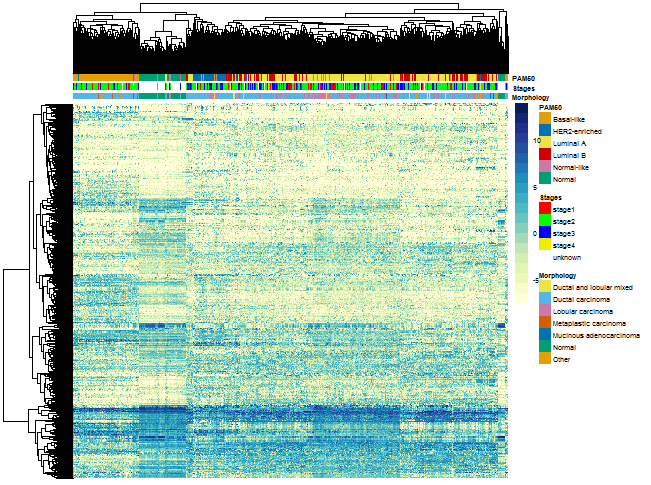
\includegraphics[scale=0.71]{heatmap_top1k.png}
            \caption[Heatmap clustering of top genes with highest variance]{Heatmap representation of clustering top 1000 highest variance genes (calculated on cancer samples only). The data is clustered by columns (samples) and rows (genes), with dendograms showing how clusters are formed. The colour bars above the heatmap (PAM50, stages, morphology) show the subgroups to which each sample belongs, colour-coded according to the legend on the right. The colours of heatmap represent gene expression magnitude according to the scale (high expression - dark blue, low expression - light yellow). The data was clustered with Euclidean distance and average linkage. }
            \label{fig:heatmap1k}
            \end{figure}
    \newpage
    First and foremost, the unsupervised clustering was able to form two main clusters: Luminal and non-Luminal samples. Cluster on the right contains the majority of Luminal A and Luminal B samples according to the top colour bar (PAM50). The left hand side cluster contains Basal-like, HER2-enriched, and normal samples. Normal samples have a distinct tanscriptomic profile which is seen from the heatmap. Normal-like subtype is scattered across the entire dendogram, with more pronounced appearance amongst Luminal A and normal samples, as expected. The Basal-like subtype cluster is well-defined, which highlights its uniqueness and distinction from the rest. The Luminal types are mixed as anticipated. Overall, clustering is in agreement with the PCA results for PAM50 subtypes. \\    
    Regarding the stages and morphology colour bars, it can be observed that clustering, much like PCA, was not able to find any distinct patterns among their subgroups. Again, the sizes of the subgroups may partially be responsible for that. It is a challenge to spot the minority-sized subgroups on the colour bar, and very clear to see how Ductal carcinoma dominates the dataset (light blue, bottom bar). The colour bar of stages also shows no distinct patterns. \\
    
    An additional exploratory clustering analysis was done to investigate the relationship between cancer stages and the underlying PAM50 subtypes. As stages of cancer progression are of great interest in this project, the averages of each PAM50 subtype at each stage were taken and clustered. Figure \ref{fig:dendogram} shows the resulting dendogram. 
    
        % dendogram
            \begin{figure}[!h]
            \centering
            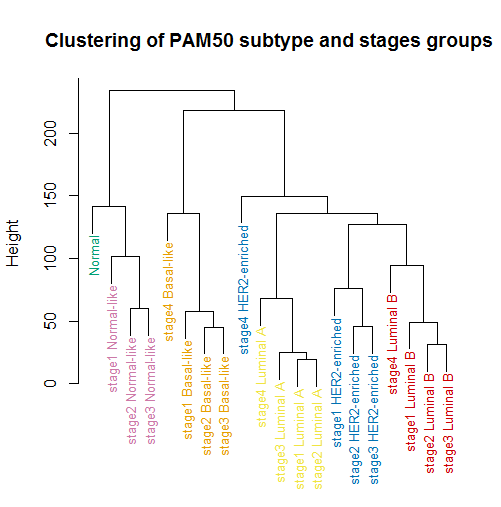
\includegraphics[scale=0.45]{dendogram2.png}
            \caption[Dendogram of PAM50 and stage subgroups clustering]{Dendogram showing clustering of PAM50 subtypes within stages (averages per stage per subtypes).}
            \label{fig:dendogram}
            \end{figure}
    
    Remarkably, all subtypes form distinct branch clusters (expect HER2-enriched). Normal and Normal-like samples are the outgroup, understandably, and then Basal-like subtype is also an outgroup to the rest of samples. Luminal types and HER2-enriched are separated to well-defined branches. It is important to note that each subtype cluster has stage 4 branch as an outgroup, with the exception of HER2-enriched stage 4, which is only made up of 2 samples perhaps leading to an unstable average. Seeing stage 4 as an outgroup is an important observation, as it is the most different and severe stage of cancer progression. \\
    
    Lastly, seeing the samples cluster primarily by PAM50 and only then by stage in Figure \ref{fig:dendogram}, is yet another evidence to what was observed with PCA and heatmap clustering. PAM50 classification is the main driving force of breast cancer samples separation. When using other classification methods, PAM50 subtypes have to be taken into account. For example, comparing two morphologies might not produce truthful results if their PAM50 subtype sample composition is the main driving effect of differences. Therefore, the heterogeneity of groups has to be taken into account, and the downstream analysis has to be done on sub-subgroups.  
    

    
    \newpage
    \subsection{Cofactors and batch effects}
    
    Morphology, cancer stages, and PAM50 molecular subtype are the anticipated sources of variation in the dataset, and namely, biological variation. However, in a large and heterogeneous dataset such as TCGA-BRCA there are several other potential sources of variation, which may be contributing to the differences in gene expression between samples. The abundance clinical and meta annotation available for the present samples allows these potential sources of technical variation to be explored.
    
    Among the available annotations, the ones of the most interest are the patient age group, year sample was taken, and tissue source site. They were explored with PCA to visualise any outlying subgroups and check for the presence of unwanted batch effects among samples, such as differences caused by being processed in different years and across a variety of research labs.
    
    One-dimensional PCA plots were used to visualise variation over the years and across the sample processing sites. As there are many ($>20$) subgroups in both year and site data, 2D PCA scatter plots are not helpful for spotting outlying subgroups. 
    
    Figure \ref{fig:1dpcayear} shows the first 6 PCs of from PCA results based on year data. Each box plot represents samples taken in a single year, with individual years shown as gitter-dots to visualise each year group approximate size and sample variation within it (according to y-axis). The box plots are shown for years in sequential order (1988-2013). \\
  
        
            % 1D PCA YEAR
            \begin{figure}[!h]
            \centering
            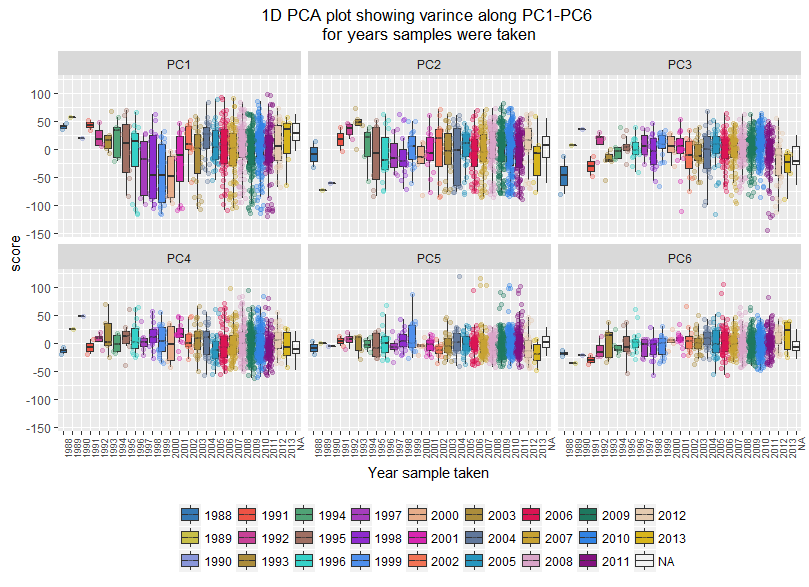
\includegraphics[scale=0.45]{1dpcayear.png}
            \caption[1D PCA plot based on year data]{One-dimensional PCA plots showing variance along PC1-PC6 for all samples (cancer and normal) taken in years 1988-2013. The dots across each box plot represent samples and their variation on the y-axis scale, to give a better indication of year group size and sample variation within it}
            \label{fig:1dpcayear}
            \end{figure}
    
    %\vspace{10mm}
    Overall, it is evident that there is a lot of variation between the years. This is especially the case for the earlier years, however, this is partially due to low number of samples taken in those years.  The variation stabilises after year 2005, which can be explained by the fact that this is when the pilot of TCGA \cite{OverviewTCGA} project started and the universal protocols were introduced. Also it can be seen that the majority of samples were collected after that time point, at the density of points is higher. Another aspect worth noticing is that samples in years 1997-2000 appear to be quite different to previous and following years (PC1). This potentially confounding effect was explored further. \\
    \newline
    
    \newpage
    As previously established, PAM50 subtypes is expected to be the main point of interest for further investigation, therefore, it is important to check the PAM50 composition of every year group to make sure that, for example, a particular subtype was \textit{not} collected in only one year, which would be confounding the dataset for further exploration. Figure \ref{fig:baryear} shows the stacked barplot of all sample counts organised by year. Each bar shows the total count of samples per year, and the proportions of samples representing each PAM50 subtype are coloured according to the legend. \\
    \newline
    
    
             % bar per year
            \begin{figure}[!h]
            \centering
            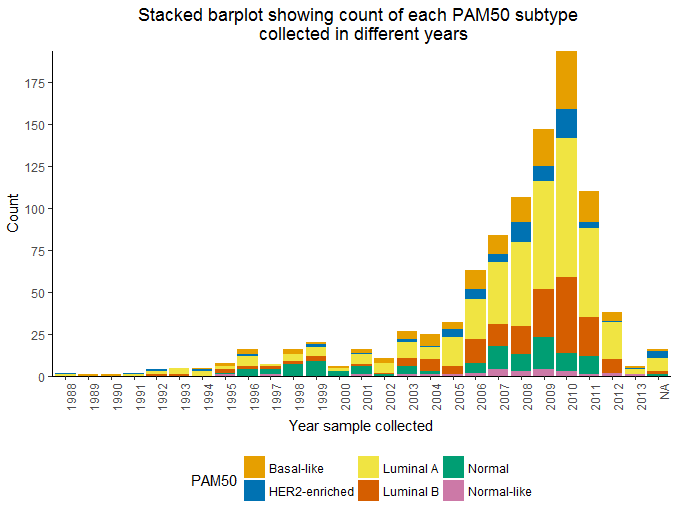
\includegraphics[scale=0.7]{bar_year.png}
            \caption[Stacked barplots of sample counts per year]{Stacked barplots of sample counts per year (1988-2013). The coloured proportions represent PAM50 subtypes samples within each year group. }
            \label{fig:baryear}
            \end{figure}
    
    As already noted from 1D PCA plot for year data, the total number of samples in the earlier years is marginally smaller than in the last decade. Overall, the distribution of PAM50 subtypes in each year is well-balanced,  although some years inevitably have no normal samples and/or samples of a specific subtype. On the whole, it can be concluded that the dataset is not confounded by a particular year-subtype combination.  
    
    Moreover, visualising data in this way has shed light on the abnormality in years 1997-2000 seen in 1D PCA plot (Figure \ref{fig:1dpcayear}, PC1). It can be seen in Figure \ref{fig:baryear} that these years are represented by $\approx50\%$ of normal samples, which is not the case for all other years. Having such high proportion of normal samples, makes their box plots to be shifted down compared to the rest, and hence appear different. Appendix \ref{} shows a 1D PCA plot for cancer samples only, confirming this explanation, i.e. years 1997-2000 do not stand out from the rest if only cancer samples are included in the analysis. \\
    

    As with year data, the sample source data was also explored with PCA and variation between different sources assessed. A 1D PCA plot (PC 1-6) showing variation for all samples grouped by samples source site (24 sites in total) is displayed in Figure \ref{fig:1dpcatss}. 
    
            
            % 1D PCA YEAR
            \begin{figure}[!h]
            \centering
            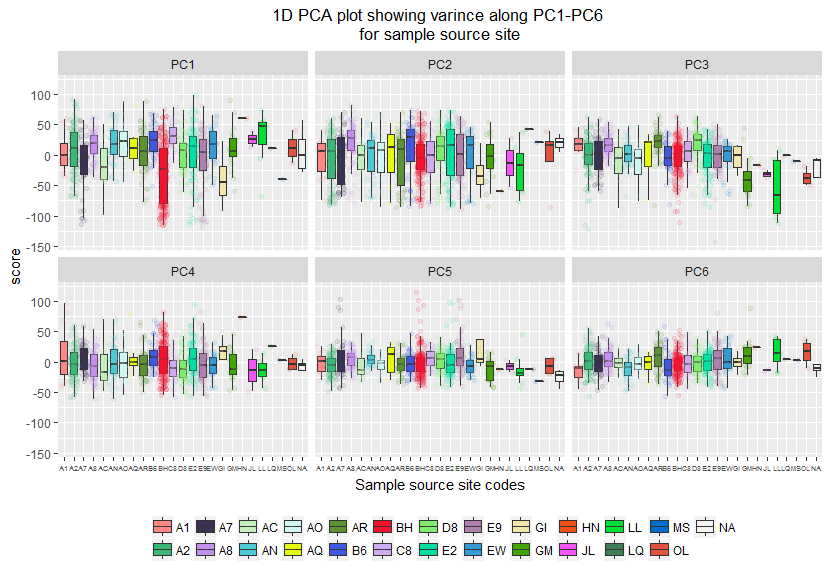
\includegraphics[scale=0.45]{1dpcatss.png}
            \caption[1D PCA plot based on sample source site data]{One-dimensional PCA plots showing variance along PC1-PC6 for all samples (cancer and normal) from different source sites (two-letter abbreviations in alphabetic order; NA - site unknown). The dots across each box plot represent samples and their variation on the y-axis scale, to give a better indication of year group size and sample variation within it.}
            \label{fig:1dpcatss}
            \end{figure}
            
            
    \newpage
    The existence of variation between source sites is unmistakably there. As with year data, some source site groups contain very few samples, which makes the variation between them and the large groups more prominent. One source site that really stands out is BH (red), PC1. A possible explanation to this observation, which would make the dataset unusable, could have been the unexpected difference in the handling protocol at this site. However, fortunately this was not the case.  \\
    
              % bar per tss
            \begin{figure}[!h]
            \centering
            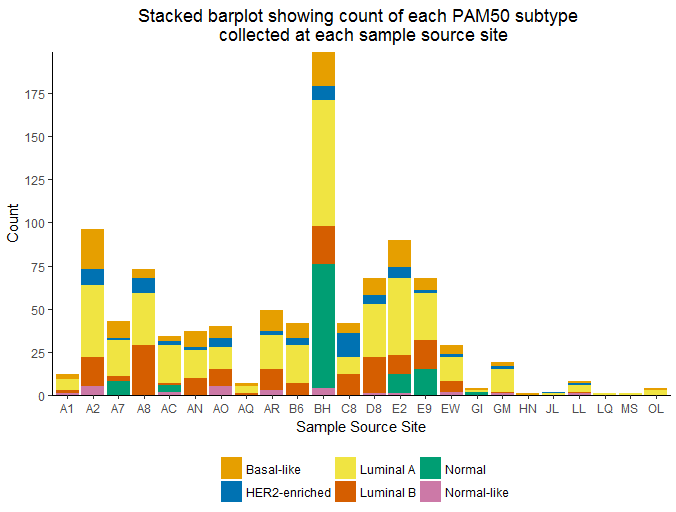
\includegraphics[scale=0.65]{bar_tss.png}
            \caption[Stacked barplots of sample counts per year]{Stacked barplots of sample counts per source site (alphabetic order). The coloured proportions represent PAM50 subtypes samples within each year group. }
            \label{fig:bartss}
            \end{figure}
    
    The source site data was visualised as stacked bar plots to inspect sample subtype variety coming from each site, Figure \ref{fig:bartss}. As observed on the 1D PCA plot, some sites have very few samples coming from them. The larger groups are relatively well-balanced in terms of their PAM50 subtype composition, with the exception of Normal-like, which comes only from 7 sites. This is, however, expected, as there are only 26 Normal-like samples in total. Another observation, which may be of bigger concern, is that the majority of normal samples come from one site, BH. This should not affect downstream analyses, as we are interested in differences between cancer subgroups. But seeing this explains the abnormal variation seen in 1D PCA plot for this site. As with year data, this one site is ~50\% composed of normal samples, making it appear very different from the rest as a group. If analysis is done only on cancer samples, this is no longer the case (Appendix \ref{}). 
    
  
    
        %data was preprocessed as described in methods
    
    
    % The outcome of the EDA will have a major impact on how you analyze the data:
    %  – Sample outliers and noise: Should some samples be discarded?
    % Can I perform a meaningful test for different expression between different groups?
    % What factors (wanted/unwanted, observed/unobserved) should be included in the model?
    
    % • EDA is the first part of the analysis where you start drawing biological conclusions specific to a
    % given experiment.
    % – Does the data look like I expected/designed?
    % – Do I have batch effects?
    % – Subgroups?
    % • In DE you formalize your observations in the EDA to extract statistically valid results.
    % • The resulting DE analysis will serve as the foundation of biological interpretation of the data.


    
    %age groups
    
    \subsection{Summary}
    
\newpage
\section{Identifying Autophagy Signatures}

    \subsection{Differential Expression Analysis}
    
    Differential expression (DE) analysis was performed on the final dataset which included 857 tumour and 112 normal samples. After all filtering steps the dataset included 15784 genes, 1090 of which were autophagy-related genes. 

    Limma-voom method was used to quantify differential expression between the samples representing subgroups of the main breast cancer classification methods (PAM50 molecular subtypes, cancer stages, tumour morphology). The subgroups are described in Section 2.1.3.4 and the number of samples per subgroup in the final dataset are presented in Tables \ref{table:morphstage} and \ref{table:pam50counts}. Figure \ref{fig:deaworkflow} shows the outline of DE analysis workflow. 

       
    % DEA workflow
            \begin{figure}[!h]
            \centering
            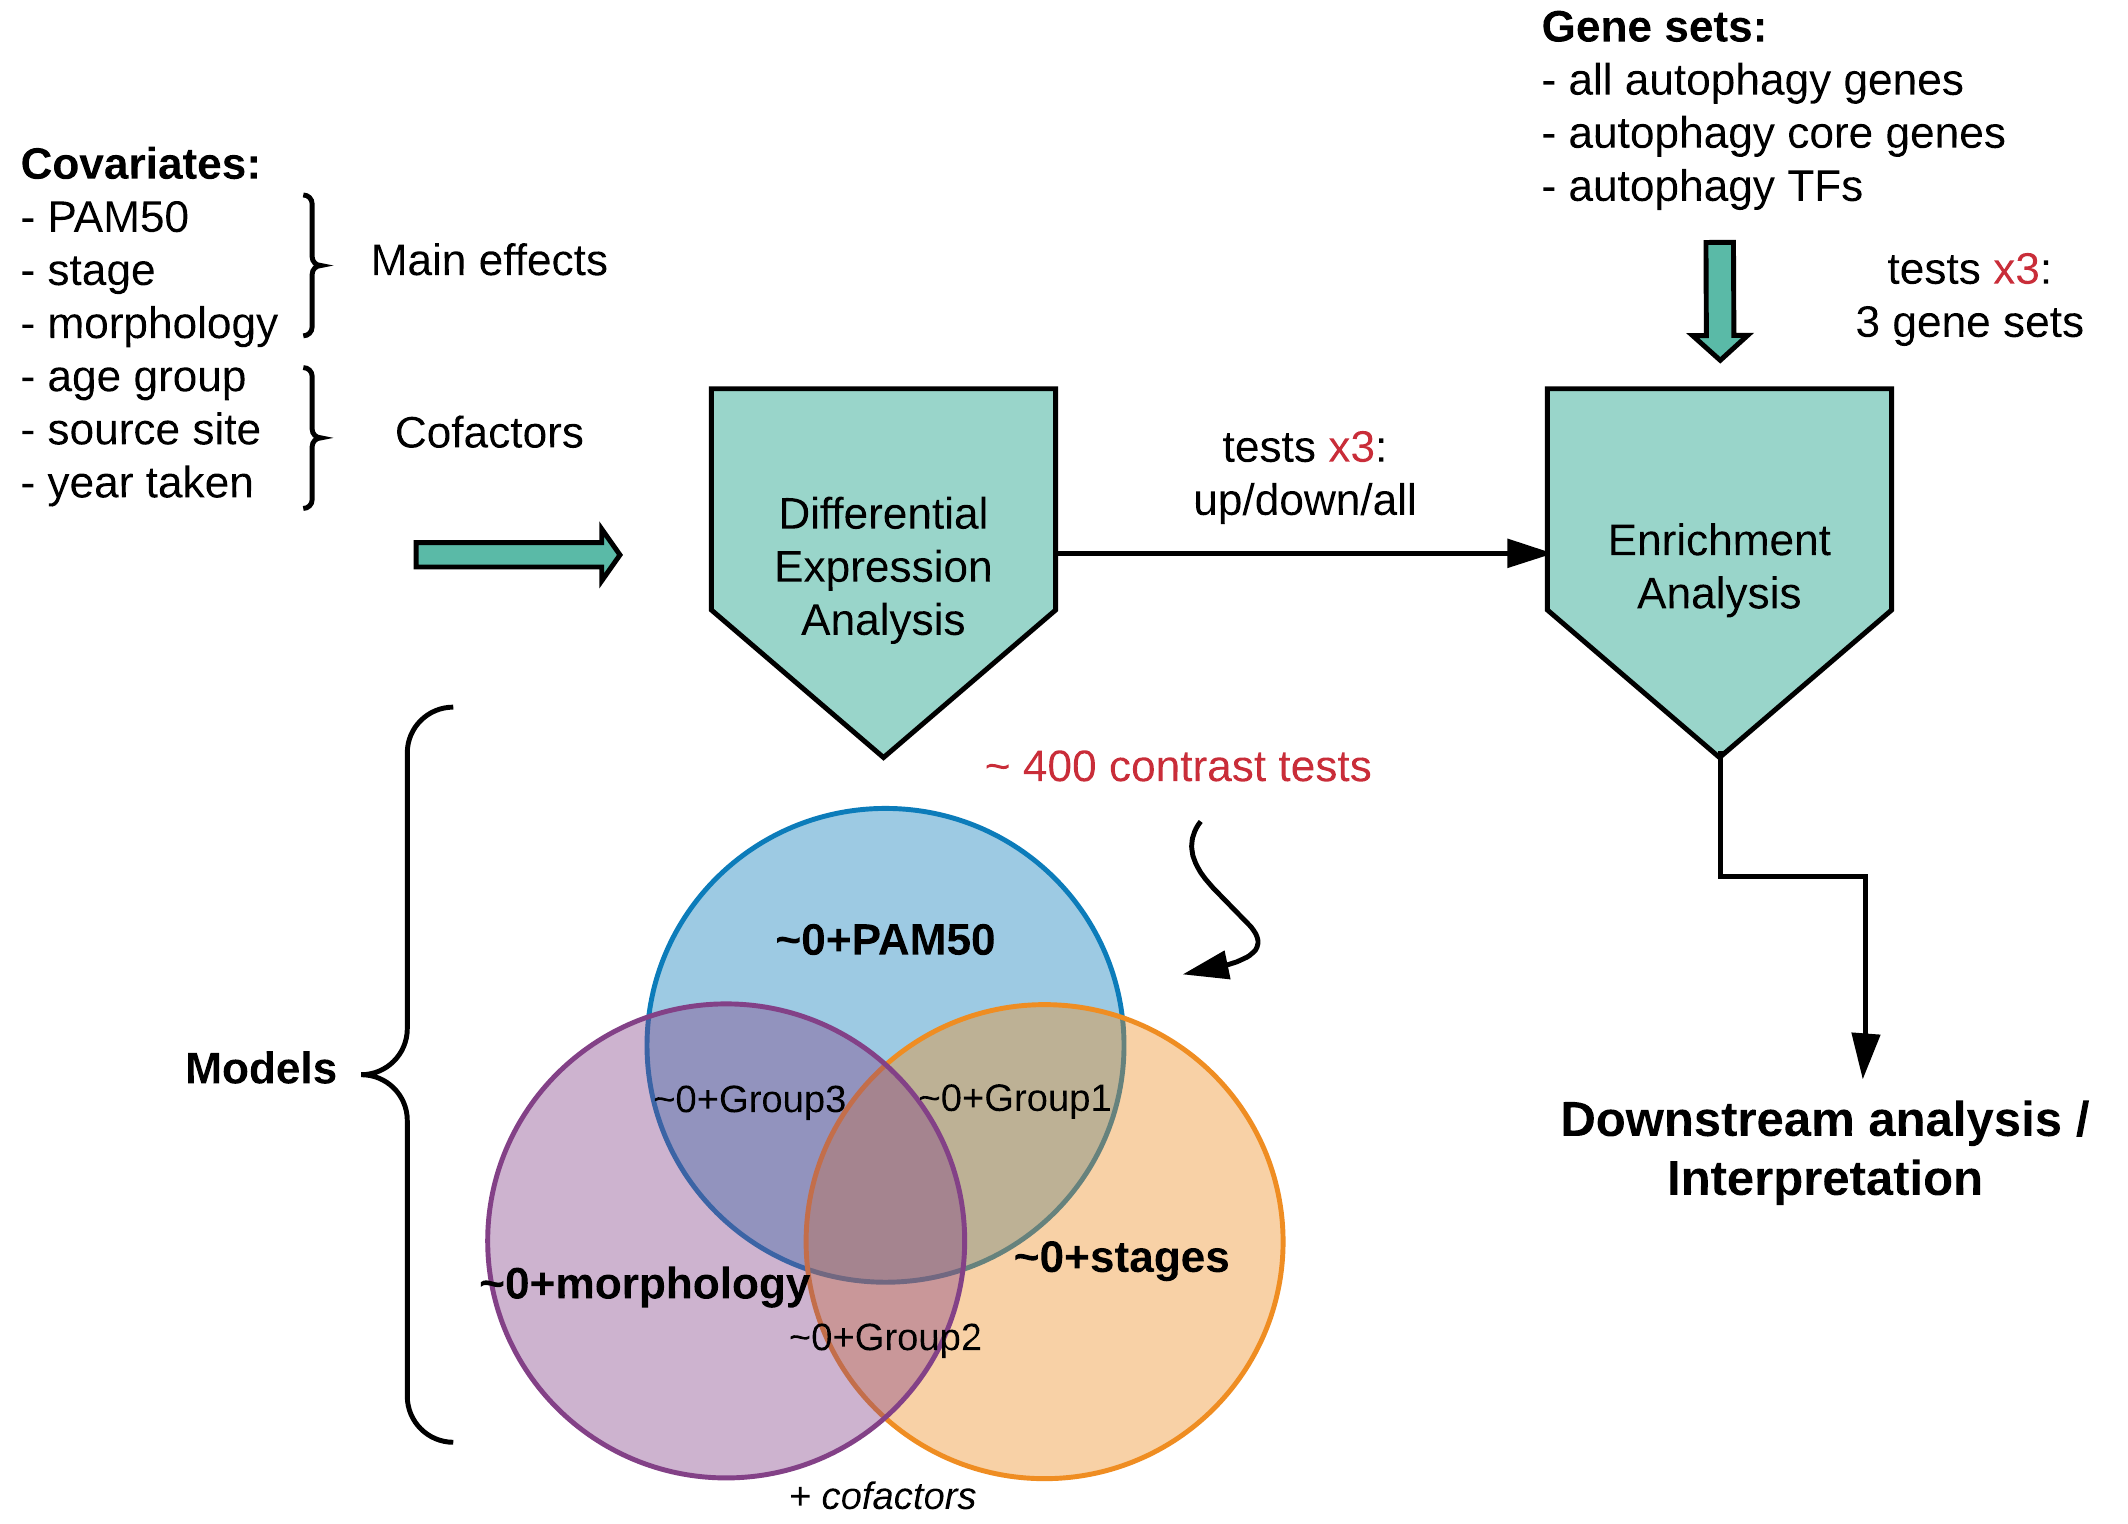
\includegraphics[scale=0.2]{dea_workflow.png} 
            \caption[Differential Expression Analysis workflow]{Differential Expression analysis workflow for the TCGA-BRCA dataset. The main classification groups/effects (PAM50, stages, morphology) as well as additional cofactors (age group, sample source site and year) were included in the models for differential expression testing. The Venn diagram shows the six tested models; the outer sections show the three main effect models, and the overlapping ‘Groups' show the three models of combined main effects. In total, $\approx 400$ contrasts across the six models were made to test for DE expression. For enrichment analysis, three gene sets were used (all autophagy genes (1090), core only (155), and TFs only (97)). Enrichment was tested in all DE genes, and also in the groups of up- or downregulated genes only. In total, 400x3x3 tests were made prior to downstream analysis.  }
            \label{fig:deaworkflow}
            \end{figure}

        \subsubsection{Main Effect Models}
        
        Each of the main sample classifications groups (PAM50, stages, morphology) were used as the main effect in individual models for DE testing. For each main effect, all combinations of subgroups and normal samples were included in the contrast matrix. In this way, for each PAM50 subtype (or each stage and morphology) differentially expressed genes were identified compared to the rest of subtypes and the normal samples. All models included the age group covariate as well as the two sources of batch effect: year and site. The raw numbers of differentially expressed genes in each contrast are available from Appendix X.

        Differential expression testing based on PAM50 subgroups has detected a fairly large number of differentially expressed genes (DEGs) in each comparison (min 5\% - Luminal A vs Luminal B, max 31\% - Basal-like vs Normal). Understandably, more of DEGs were found in contrasts with normal samples, with a noticeably larger proportion being downregulated in cancer samples. The proportions of DE-regulated genes between PAM50 subtypes ranged between 5\% and 22\% (Luminal A vs Luminal B and Luminal A vs Basal-like), and a subtype vs normal 12\% (Normal-like) to 31\% (Basal-like). 
        
        Differential expression testing based on cancer stages showed a considerable number of differentially expressed genes between stages and normal samples, $\approx 23\%$ at each stage. Interestingly, the analysis has found only very few genes to be DE between individual stages.
        
        Differential expression testing based on tumour morphology showed that the most DEGs-rich contrasts are again the ones with the normal samples. In the contrasts of morphology types compared to normal samples the proportion of DEGs varied between 21\% and 28\%. The two main morphologies, Lobular and Ductal carcinomas,  had only 6\% (924) DEGs between them. When both were tested with the mixed Lobular+Ductal morphology, both had less than 20 DEGs, meaning that this morphology is too much of a blend between the two separate ones to detect sufficient differential expression. Metaplastic and Mucinous morphologies were found to have the most DEGs with Lobular morphology (15\% and 13\%), and less with Ductal (6\% and 9\%) and Lobular+Ductal (10\% and 6\%) morphologies. The largest number of DEGs between two morphologies was between Metaplastic and Mucinous - 19\%. 
        
        Overall, large numbers of differentially expressed genes between PAM50 subtypes is an expected and reassuring result, as it is known from exploratory analysis that the differences between them is the strongest source of variation in the data. Not being able to see many differentially expressed genes between stages can be due to heterogeneity of the dataset, which is also probably contributing to differential expression in morphology types. %As noted previously with the PCA of morphology, the two types that show a clear separation (Metaplastic and Mucinous) are likely to be driven so by their exclusivity of PAM50 sample composition. Therefore, a large number of differentially expressed genes between them is also a likely consequence of that. 

        \subsubsection{Combined Effect Models}
        
        The reduce the effect of data heterogeneity in the differential expression analysis, additional models with combined groups effect were tested. Three models were created: PAM50 + stage (Group1), morphology + stage (Group2), PAM50 + morphology (Group3), as shown in Venn diagram in Figure \ref{fig:deaworkflow}. This analysis setup allowed testing for differential expression in more precisely defined groups,  for example, Group1 model is able to quantify expression between stages of a specific subtype, i.e. between stages 1 and 2 of Luminal A. Again, all models included the age group, year, and source site as cofactors.

        In general, a large number of separate PAM50 subtype-specific differentially expressed genes were found at individual stages and in specific morphologies. As the number of contrasts for each Group is around 100, the details will be omitted. 
        
        Differential expression analysis with Group1 model (PAM50 + stage) has shown that all subtypes at all stages have a large number of DEGs compared to normal samples. Between different stages of a single subtype, only Basal-like and Luminal B had a reasonable number of DE genes. Contrasts between the same stages of different PAM50 subtypes have shown that Luminal A and Basal-like have the largest number of differentially expressed genes consistently at all stages. Interestingly, at stage 4 there was the smallest numbers of differentially expressed genes between subtypes. 
        
        Differential expression analysis with Group2 model (stage + morphology) has shown that Ductal morphology has the largest number of DEGs at all stages. Ductal is the only morphology that contains stage 4 samples in this dataset, so the comparisons for the rest of morphologies were made based only on first three stages. The stage-wise comparison of Lobular and Ductal carcinomas has shown that the number of DEGs between them increases with stage. This seems reasonable, as both of them have a adequate number of samples per stage, and also both are represented by a good mix of PAM50 subtypes (Table \ref{table:counts}). \\ This is, however, not the case for contrasts involving Mucinous and Metaplastic types. As mentioned before, their PAM50 composition is restricted to Luminal and Basal subtypes, respectively, which makes all comparisons made with them dubious, as the true variation driving force is unknown. The DE results between the two have shown a very large number of differentially expressed genes, particularly at stage 2. There, the comparison that is being made is only between 4 and 5 samples, which are exclusively Basal-like and Luminal A. In an earlier comparison these two subtypes showed the highest number of DEGs on the all-samples level, and here, this compelling difference appears to be maintained at the level of a few samples too. 
        \newpage
        Differential expression analysis with Group3 model (PAM50 + morphology) is of interest mostly only for Lobular and Ductal morphologies, as they contain enough samples to represent each PAM50 subtype (Table \ref{table:counts}). Both have a large number of differentially expressed genes between all subtypes, with Ductal carcinoma having a distinctly large number for the contrast between Luminal A and Basal-like.  \\

        \subsubsection{Enrichment Analysis}
        
        Ultimately, we are interested not in the numbers of differentially expressed genes in each contrast per se, but in whether these subsets of DEGs are enriched for autophagy-related genes. As shown in the diagram in Figure \ref{fig:deaworkflow}, groups of up-, down-, and both direction regulated genes were tested for enrichment. Three separate gene sets were used in the Fisher’s test - all autophagy genes, only autophagy core genes, and only autophagy-related transcription factors (TFs). The significance of autophagy enrichment was evaluated based on the cut-off for adjusted p-value ($<0.05$) and the odds-ratios score ($>1$). The results significant at non-adjusted p-value were also considered.

        However, the enrichment results have largely been unfruitful, particularly on the differential expression results from the individual main effect models. The raw data is shown in Appendix X2. 
        
        For the individual main effect models (only PAM50, stage, or morphology) none of the subsets of differentially expressed genes detected in contrast tests have been assigned an odds-ratio $>1$ and simultaneously been significant at adjusted p-value level. There were several contrasts enriched for TFs but only at non-adjusted p-value, all of which were downregulation compared to normal:
        
        \begin{itemize}
            \item Luminal A, Luminal B, and Basal-like  (both directions in Luminal B)
            \item Stage 2, stage 3, and stage 4 
            \item Metaplastic, Mucinous, and Lobular+Ductal mixed \\
        \end{itemize}
        
        \vspace{5mm}
        When using Group models, i.e. combining two effects, some contrasts were found enriched at acceptable level.
        
        In Group1, ‘all autophagy’ genes were enriched in the downregulated genes at stage 4 of Basal-like subtype compared to stage 4 of Luminal A and Luminal B, and also to normal samples. At non-adjusted p-value level, there were 13 contrasts enriched for TFs downregulated in a cancer type vs normal. Among these, there was stage 1 of every PAM50 subtype, all stages of Basal-like subtype (details in Appendix X2). 
         
        In Group2, autophagy TFs were enriched in the downregulated genes in every morphology compared to normal, at varying stages. There was also a strong enrichment in TFs that are differentially expressed between Lobular and Ductal carcinomas at stage 1. At non-adjusted p-value level, there was a large number of contrasts enriched for autophagy TFs, mainly in the downregulated in cancer vs normal fashion. Among these are all stages of Ductal and Mucinous types, as well as stages 1 and 3 of Metaplastic. Interestingly, Lobular carcinoma did not appear in this context at all. Nonetheless, groups of upregulated genes in Lobular compared to Metaplastic (stage 3) and Mucinous (stage 2) were enriched for autophagy (Appendix X3). 
        
        In Group3, ‘all autophagy’ genes were enriched in the downregulated genes in Basal-like samples compared to Luminal A and Normal-like samples (all of Lobular morphology) and normal samples. When looking at non-adjusted p-value, Luminal B can also be added to this pattern. For non-adjusted p-value enrichment for TFs, there were multiple enriched contrasts, again including several instances of downregulation in cancer vs normal (particularly Basal-like and Luminal B), DE between morphologies within Basal-like subtype, and again similar for Lobular carcinoma as for ‘all autophagy’.
        
        \newpage
        Overall, it seems that using the combined main effects models allows to detect more autophagy enrichment in the differential expression results. As only specific combinations of samples are considered, the heterogeneity is decreased, allowing for a stronger differential expression signal, i.e. more genes are reported. However, it still cannot be claimed that enrichment results attained from the combined models provide strong evidence of a particular group of samples being enriched for autophagy. Hence, the main observations are:
        
        \begin{itemize}
            
        \item The main reoccurring trend among all tested contrasts of differentially expressed genes is autophagy enrichment among genes that are being downregulated in cancer. 
        \item There is a consistent enrichment for autophagy TFs in genes downregulated in separate stages/morphologies (at adjusted and non-adjusted p-value level)
       \item There is not autophagy enrichment in genes that are differentially expressed between stages. This is the case for both the main effect model, and the models with stage combined with other subgroups.

       \item Among the frequently seen potentially enriched groups of samples are Basal-like subtype, Lobular morphology, stage 4.  However, exploring these groups further cannot be justified, as there are very few samples in them. Table \ref{table:counts} shows that stage 4 samples are available only for Ductal morphology, and of samples that are Basal-like and have Lobular morphology there are only 3. 

        
        \end{itemize}
        \subsubsection{Summary}
        
        Differential expression analysis of the TCGA-BRCA dataset was performed based on three sample classification methods -- stage, morphology, PAM50 molecular profile. The analysis involved around 400 differential expression tests across six model. The results have shown that contrasts between samples classified by their molecular profile detect the largest amount of DEGs, both when using the model with a single main effect and models with combined effects. Conversely, very minimal (if any) differential expression was detected between cancer stages, both with single main effect model and models with combined effects. With morphology classification, the most DEGs-abundant contrast was between two smallest in size mophologies, Metaplastic and Mucinous. Considerably less DEGs were found between the two main morphologies, Ductal and Lobular. However, much more differential expression was detected between Ductal and Lobular morphologies in individual PAM50 subtypes. 
        
        Overall, enrichment analysis was unsuccessful in identifying autophagy enrichment in any of the groups of differentially expressed genes. There were several contrasts of samples changes between which included a significantly large proportion of autophagy genes and therefore were considered enriched. However, this enrichment was not consistent and usually appeared in the groups that were represented by too few samples to be reliable. The general trend for autophagy genes is downregulation in various subgroups of cancer samples compared to normal. Particularly this trend is true for autophagy-regulating transcription factors. 
        
        
        
        
        
        
        

\newpage
    \subsection{Soft clustering}
    Soft clustering was performed on all samples together to evaluate the expression patterns in the dataset as whole, and also on separate PAM50 subtypes individually to detect any molecular profile-specific patterns. Classification by morphological groups was decided not to be included in the analysis due to the underlying imbalance of PAM50 composition of each morphology, and also the fact that only one morphology contains samples of all stages (Ductal carcinoma). 

    
   
    \subsubsection{Full Dataset Clustering}
     Gene clustering results based on full dataset expression data are presented in Figure \ref{fig:mfuzzall}. The genes were grouped into six clusters according to expression changes between normal samples and cancer samples of different stages. 
     Clusters 4 and 5 represent genes that are downregulated or upregulated, respectively, in cancer compared to normal, regardless of the stage. Clusters 1 and 2 represent patterns of more gradual down- and up- regulation in cancer, with a distinct rapid change in stage 4. Clusters 3 and 6 are assigned genes that have altered expression at initial stages of cancer, while towards the most serious stage, i.e. stage 4, the expression resembles normal expression. 
     Here, only the genes with $>0.6$ cluster membership score are presented, as they are the main contributors to a cluster's stability and dominant expression pattern. Only those genes are considered in downstream analysis as cluster representatives. 

        
         % mfuzz all samples
            \begin{figure}[!h]
            \centering
            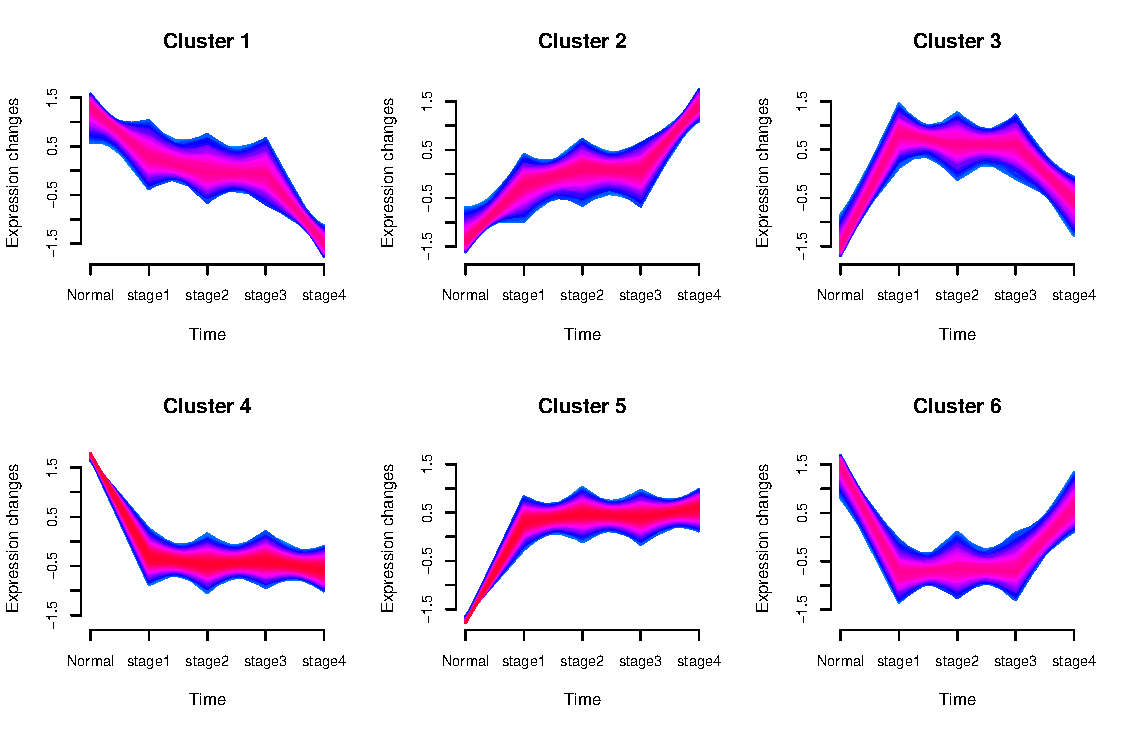
\includegraphics[scale=0.65]{mfuzz_allsamples_6cl_15k.pdf} 
            \caption[Soft-clustering results for all samples gene expression]{Soft-clustering results based on all samples data. Each cluster describes an expression change pattern (y-axis), made up by genes that follow its dominant pattern across the stages (x-axis). Genes only with membership score $>0.6$ are shown. Number of genes per cluster: 1 - 792, 2 - 1005, 3 - 796, 4 - 3224, 5 - 2889, 6 - 743.}
            \label{fig:mfuzzall}
            \end{figure}
            
        In this way, the obtained six gene groups were tested for autophagy enrichment. As previously with differential expression results, three gene sets were used: all autophagy genes, only autophagy core genes, and only autophagy-related transcription factors (TFs). The significance of autophagy enrichment was evaluated based on the cut-off for adjusted p-value ($<0.05$) and the odds-ratios score ($>1$).
        
        Table \ref{table:mfuzzall} presents the enrichment results for clustering on all samples. For each gene set, the number of autophagy genes present in a cluster is reported, along with the odds-ratio score, p-value, and adjusted p-value. The cluster that is found to be enriched for autophagy is marked with bold (Cluster 4), at both all genes and TFs-only levels. Cluster 4 comprises the genes that are downregulated at all cancer stages compared to normal. 264 autophagy-related genes display this expression pattern, 39 of them are TFs.
    

        
            %TABLE
             \begin{table}[!h]
            \centering
            \small
            \caption[Enrichment analysis results based on soft-clustering data]{Autophagy enrichment results on soft-clustering results based on all samples. Three autophagy gene sets were tested: all genes, core autophagy genes, and autophagy TFs. The cluster that is significantly enriched is cluster 4. }
            \label{table:mfuzzall}
            \begin{tabular}{lcccc}
            \multicolumn{1}{l|}{} & \multicolumn{1}{l|}{\textbf{n genes}} & \multicolumn{1}{l|}{\textbf{odds-ratio}} & \multicolumn{1}{l|}{\textbf{p-value}} & \multicolumn{1}{l}{\textbf{adj. p-value}} \\ \hline
            \multicolumn{5}{l}{\textit{all autophagy genes}} \\ \hline
            \multicolumn{1}{l|}{cluster1} & \multicolumn{1}{c|}{47} & \multicolumn{1}{c|}{0.84} & \multicolumn{1}{c|}{0.31} & 0.63 \\ \hline
            \multicolumn{1}{l|}{cluster2} & \multicolumn{1}{c|}{69} & \multicolumn{1}{c|}{0.99} & \multicolumn{1}{c|}{1} & 1 \\ \hline
            \multicolumn{1}{l|}{cluster3} & \multicolumn{1}{c|}{51} & \multicolumn{1}{c|}{0.92} & \multicolumn{1}{c|}{0.61} & 0.92 \\ \hline
            \multicolumn{1}{l|}{\textbf{cluster4}} & \multicolumn{1}{c|}{264} & \multicolumn{1}{c|}{1.26} & \multicolumn{1}{c|}{2e-03} & 7e-03 \\ \hline
            \multicolumn{1}{l|}{cluster5} & \multicolumn{1}{c|}{150} & \multicolumn{1}{c|}{0.69} & \multicolumn{1}{c|}{4e-05} & 2e-04 \\ \hline
            \multicolumn{1}{l|}{cluster6} & \multicolumn{1}{c|}{53} & \multicolumn{1}{c|}{1.04} & \multicolumn{1}{c|}{0.76} & 0.92 \\ \hline
            \multicolumn{5}{l}{\textit{autophagy core genes}} \\ \hline
            \multicolumn{1}{l|}{cluster1} & \multicolumn{1}{c|}{4} & \multicolumn{1}{c|}{0.49} & \multicolumn{1}{c|}{0.19} & 0.42 \\ \hline
            \multicolumn{1}{l|}{cluster2} & \multicolumn{1}{c|}{8} & \multicolumn{1}{c|}{0.79} & \multicolumn{1}{c|}{0.74} & 0.89 \\ \hline
            \multicolumn{1}{l|}{cluster3} & \multicolumn{1}{c|}{9} & \multicolumn{1}{c|}{1.16} & \multicolumn{1}{c|}{0.58} & 0.87 \\ \hline
            \multicolumn{1}{l|}{cluster4} & \multicolumn{1}{c|}{32} & \multicolumn{1}{c|}{1.01} & \multicolumn{1}{c|}{1} & 1 \\ \hline
            \multicolumn{1}{l|}{cluster5} & \multicolumn{1}{c|}{22} & \multicolumn{1}{c|}{0.73} & \multicolumn{1}{c|}{0.21} & 0.42 \\ \hline
            \multicolumn{1}{l|}{cluster6} & \multicolumn{1}{c|}{13} & \multicolumn{1}{c|}{1.87} & \multicolumn{1}{c|}{0.05} & 0.31 \\ \hline
            \multicolumn{5}{l}{\textit{autophagy TFs}} \\ \hline
            \multicolumn{1}{l|}{cluster1} & \multicolumn{1}{c|}{7} & \multicolumn{1}{c|}{1.48} & \multicolumn{1}{c|}{0.34} & 0.41 \\ \hline
            \multicolumn{1}{l|}{cluster2} & \multicolumn{1}{c|}{2} & \multicolumn{1}{c|}{0.31} & \multicolumn{1}{c|}{0.09} & 0.19 \\ \hline
            \multicolumn{1}{l|}{cluster3} & \multicolumn{1}{c|}{5} & \multicolumn{1}{c|}{1.02} & \multicolumn{1}{c|}{0.82} & 0.82 \\ \hline
            \multicolumn{1}{l|}{\textbf{cluster4}} & \multicolumn{1}{c|}{39} & \multicolumn{1}{c|}{2.62} & \multicolumn{1}{c|}{1e-05} & 7e-05 \\ \hline
            \multicolumn{1}{l|}{cluster5} & \multicolumn{1}{c|}{10} & \multicolumn{1}{c|}{0.51} & \multicolumn{1}{c|}{0.05} & 0.14 \\ \hline
            \multicolumn{1}{l|}{cluster6} & \multicolumn{1}{c|}{2} & \multicolumn{1}{c|}{0.42} & \multicolumn{1}{c|}{0.33} & 0.41 \\ \hline
            \end{tabular}
            \end{table}
        
     
        \newpage
        \subsubsection{Subtype-specific Clustering}
        
        Clustering was performed on individual PAM50 subtype samples to evaluate the presence of any characteristic expression patterns and test for subtype-specific autophagy enrichment. 
        For individual subtypes, figures with complete set of clusters and enrichment results tables can be found in Appendix X3. Here, only selected cluster details are presented. 
        
        
        \begin{wrapfigure}{R}{0.28\textwidth}
        \hfill
        \captionsetup{justification=centering}
        \centerline{ 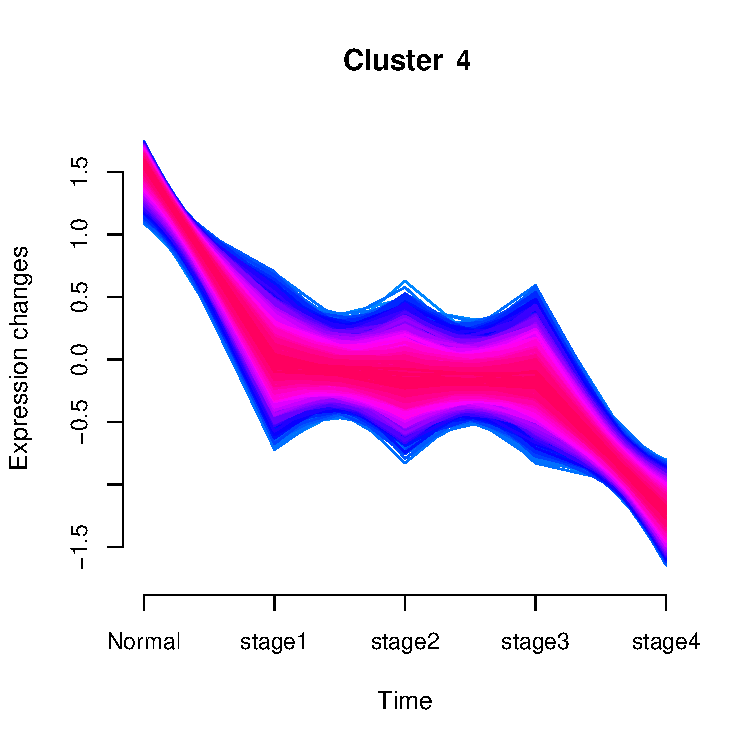
\includegraphics[width=0.24\textwidth]{mfuzz_basal_enriched_cluster.pdf}}
        \vspace*{-8mm}
        \caption[Basal-like subtype downregulation cluster]{\label{fig:mfuzzbasal}Basal-like\newline downregulation cluster}
        \end{wrapfigure}

        
        \textbf{Basal-like subtype}\\
        The expression patterns of Basal-like samples are different from the full dataset patterns. There are no clusters with strict up- or downregulation trend in cancer, instead, there are patterns with additional up- or downregulation in stage 4 (Appendix X3; Clusters 1 and 4). Additionally, there are two new patterns, in which the expression is the same in normal and stages 1-3, but drastically up- or downregulated in stage 4 (Appendix X3; Clusters 2 and 6).  
        Autophagy is enriched in Basal-like samples also in the pattern of downregulation in cancer (Cluster 4, individual cluster is shown in Figure \ref{fig:mfuzzbasal}), but the pattern has extra downregulation at stage 4. Cluster 4 contains 177 autophagy genes, and enrichment is defined by odds-ratio score 1.25 and adjusted p-value 0.03. 
        
        
        \begin{wrapfigure}{R}{0.28\textwidth}
        \hfill
        \captionsetup{justification=centering}
        \centerline{ 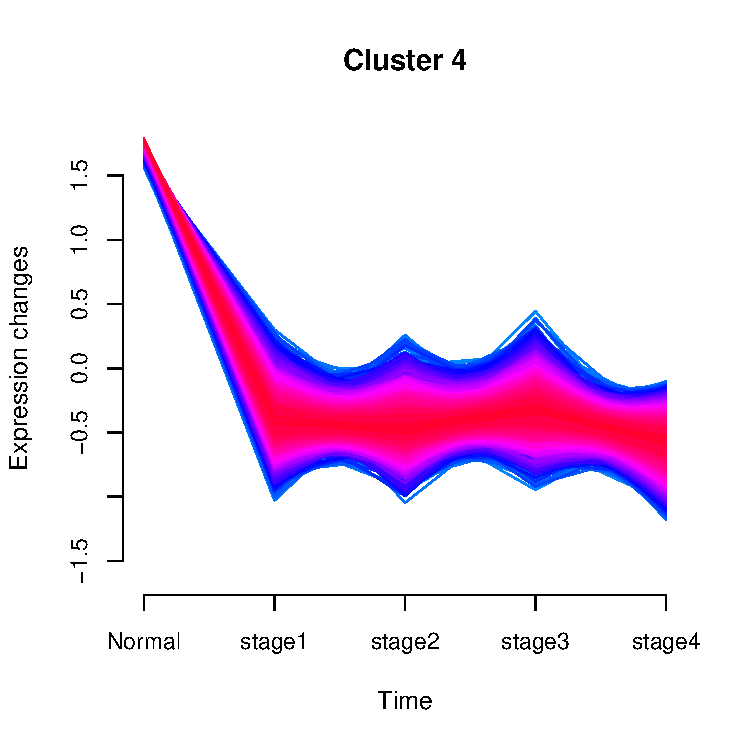
\includegraphics[width=0.24\textwidth]{mfuzz_lumA_enriched_cluster.pdf}}
        \vspace*{-8mm}
        \caption[Luminal A subtype downregulation cluster]{\label{fig:mfuzzluma}Luminal A \newline downregulation cluster}
        \end{wrapfigure}
        
        
        \textbf{Luminal A subtype}\\   
        The expression in Luminal A samples is similar to the all-samples pattern. There are clusters with exclusive up- and downregulation in all cancer stages (Appendix X3; Clusters 3 and 4). There are also clusters with the patterns observed in Basal-like -- relatively unchanged expression until stage 3, and then rapid raise/drop in stage 4. In Luminal A, however, downregulation cluster (Figure \ref{fig:mfuzzluma}) is not found to be enriched for autophagy at ‘all autophagy genes' level, as it is with all and Basal-like samples, even though it is the most gene-abundant cluster like in the other subtypes (Appendix X3). Here, autophagy enrichment is detected only at TFs level: 36 genes, odds-ratio 2.92, adjusted p-value 1.1e-05.\vspace{-5mm} \break
        
        \begin{wrapfigure}{L}{0.28\textwidth}
        \hfill
        \captionsetup{justification=centering}
        \centerline{ 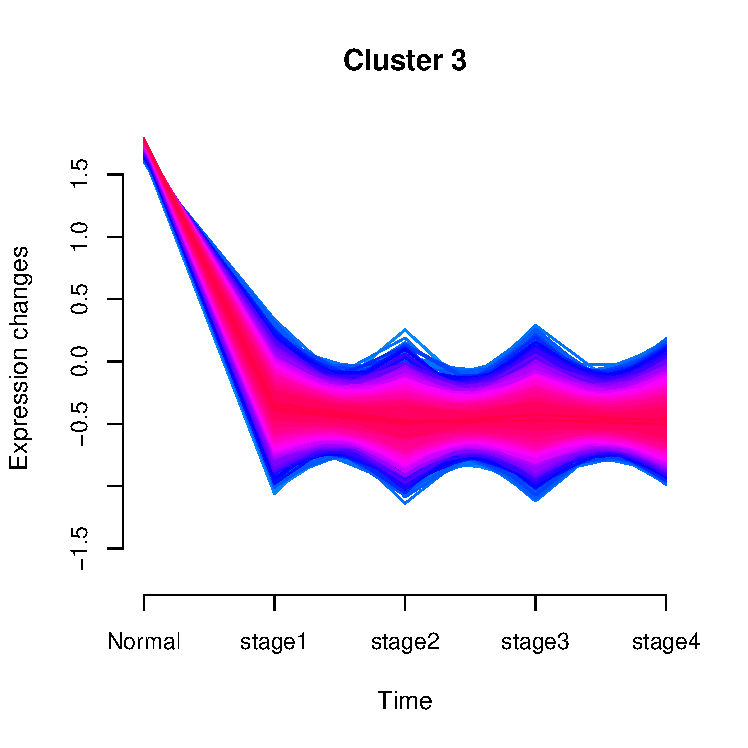
\includegraphics[width=0.24\textwidth]{mfuzz_lumB_enriched_clusterNOT_1.pdf}}
        \vspace*{-8mm}
        \caption[Luminal B subtype downregulation cluster]{\label{fig:mfuzzlumb}Luminal B\newline downregulation cluster}
        \end{wrapfigure}
        
        
        \textbf{Luminal B subtype}\\      
        The samples of Luminal B subtype have expression pattern the most similar to full dataset than all other subtypes. Again, the downregulation cluster (Figure \ref{fig:mfuzzlumb}) contains the largest number of autophagy genes, but the enrichment is only significant in TFs gene set (23 genes, odds-ratio 2.15, adjusted p-value 0.01). 
        \newline
        \newline
        \newline
        \newline
        \newline

      
        \begin{wrapfigure}{L}{0.28\textwidth}
        \hfill
        \captionsetup{justification=centering}
        \centerline{ 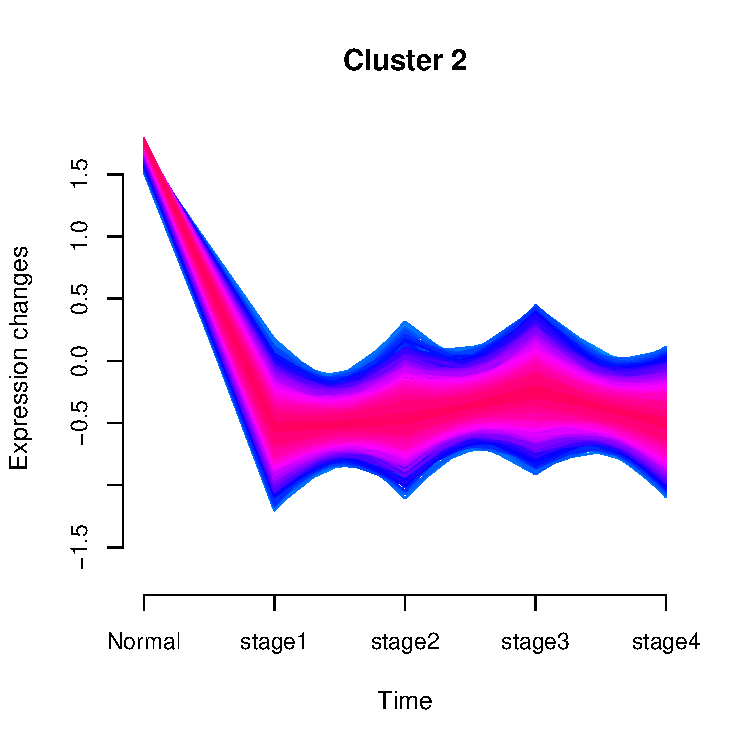
\includegraphics[width=0.24\textwidth]{mfuzz_her2_enriched_clusterNOT.pdf}}
        \vspace*{-8mm}
        \caption[HER2-enriched subtype downregulation cluster]{\label{fig:mfuzzher}HER2-enriched \newline downregulation cluster}
        \end{wrapfigure}
     
     
        \textbf{HER2-enriched subtype}\\   
        Gene clustering based on HER2-enriched samples generated overall less stable clusters. In Appendix X3 it can be seen that their cores contain less samples with high membership score (i.e. appear less ‘red'). Expression patterns are similar to the ones observed previously. Again, the downregulation cluster (Figure \ref{fig:mfuzzher}) contains the largest number of autophagy genes, but the enrichment is only significant in TFs gene set (21 genes, odds-ratio 2.13, adjusted p-value 0.02).
        \newline
        \newline
        \newline        


        
        \begin{wrapfigure}{L}{0.28\textwidth}
        \hfill
        \captionsetup{justification=centering}
        \centerline{ 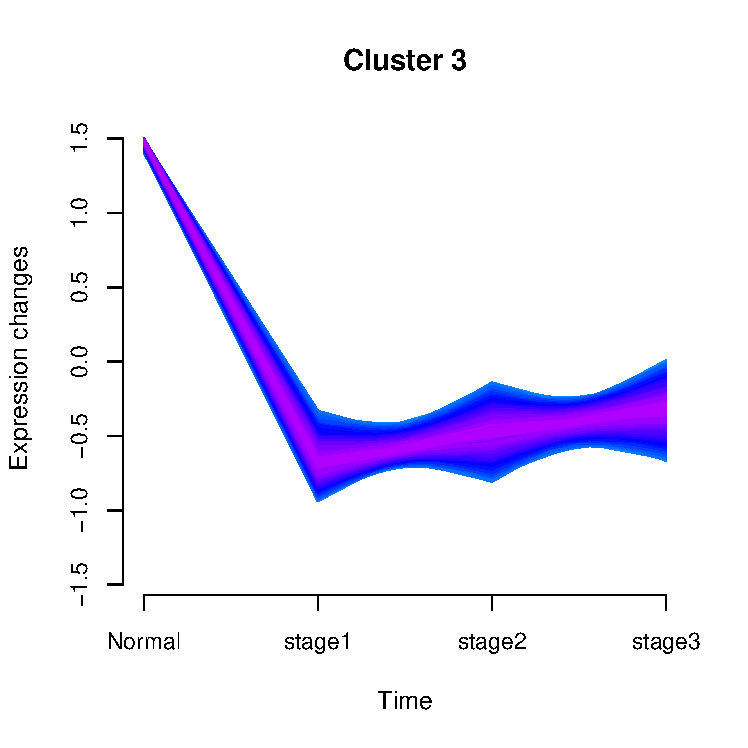
\includegraphics[width=0.24\textwidth]{mfuzz_normlike_enriched_clusterNOT.pdf}}
        \vspace*{-8mm}
        \caption[Normal-like subtype downregulation cluster]{\label{fig:mfuzznorm}Normal-like\newline downregulation cluster}
        \end{wrapfigure}
      
        \textbf{Normal-like subtype}\\ 
        Unlike other subtypes, for Normal-like subtype, there are only samples of stages 1-3 available. Clustering of these samples has produced a variety of new cluster plots not seen for other subtypes in addition to the reoccurring up- and downregulation trends. The number of genes in each cluster at $>0.6$ level is noticeably lower.  As a consequence, there is no autophagy enrichment in any of the clusters for any of the gene sets. Figure \ref{fig:mfuzznorm} shows the downregulation cluster based on Normal-like samples. 
        \newline
        \newline
        \newline
        

    \subsubsection{Summary}
    
    Overall, it seems that the downregulation trend characterises the autophagy genes behaviour the most. Both in all samples and in individual subtypes it is the largest cluster with the highest number of autophagy-related genes, and it is seen enriched at several instances. 
    
    The downregulation pattern is enriched for ‘all autophagy' gene set in all-samples group and in Basal-like subtype. Then, for ‘autophagy TFs' gene set it is enriched in all samples, Luminal A, Luminal B, and HER2-enriched subtypes. The exact pattern of downregulation cluster varies slightly between subtypes. In Luminal B the trend is ideally straight; in Luminal A and HER2-enriched the cluster has a very slight dip at stage 4; and in Basal-like it is changes between stage 3 and 4 as much as between normal and stage 1. Normal-like subtype has the weakest clusters with the least number of genes being $>0.6$ members, which is perhaps a result of having less samples in total (Table \ref{table:counts}) -- this may also be affecting HER2-enriched group. And also not having stage 4 samples, i.e. having a different number of time points, has brought out other expression patterns in Normal-like subtype. 
    
    
    

    
    %identify distinct transcriptome clusters
    %classify genes into groups
    
    %     The expression profiles of these 348 genes were sorted into 5 clusters by using the fuzzy c-means algorithm implemented in the R package Mfuzz (20). The Mfuzz package uses a “fuzzy” clustering approach to compute the strength of the association of each gene with the central behavior of the cluster, referred to as a “fuzzy score.” The fuzzy scores for each gene sum to 1. This allows one to define a set of genes that associate with each cluster with a high probability, while other genes may not have a high score for association with a single cluster but may instead have scores that allow partial placement in more than one cluster. This approach is more flexible and less sensitive to experimental noise than traditional “hard” clustering, where each gene must belong to one and only one cluster.
 
% Table S1 in the supplemental material shows each of the 348 genes assigned to the 5 clusters and their individual fuzzy scores. The median fuzzy score for each cluster was >0.98, and the average fuzzy score was >0.9, indicating strongly correlated behaviors of the genes within each cluster with respect to changes in growth rate and substrate. Thus, each cluster has a core set of genes with very high fuzzy scores (i.e., close to 1) which indicate that their collective expression behavior is strongly correlated with that of other members of the cluster with respect to their changes in growth rate and substrate. Moreover, the lack of significant overlap of genes between the clusters also supports the unique characteristics of the clusters and their embedded genes.



 
% To overcome the limitations of hard clustering, soft clustering can be applied o
% ering several advantages to researchers [1, 2]. First, it generates accessible internal cluster structures, i.e. it indicates how well corresponding clusters represent genes/proteins. This additional information can be used for a rened search for regulatory elements. Second, the overall relation between clusters, and thus a global clustering structure, can be dened. Additionally, soft clustering is more noise robust and a priori pre-ltering of genes can be avoided. This prevents the exclusion of biologically relevant genes/proteins from the data analysis.


\section{Comparative Analysis and Interpretation}

The results of differential expression analysis and soft-clustering overall agree on the fact that autophagy signature in the given dataset is observed among the genes downregulated in various breast cancer subtypes when compared to normal. Therefore, it is important to investigate the extent of this agreement both between the two methods, and also among subtypes and stages in separate results. 

\subsection{Inspecting results of two methods}

\subsubsection{Identifying subset of interest}

Gene expression clustering of individual PAM50 subtype samples has produced six clusters for each subtype, among which the downregulation trend clusters were the most autophagy genes-abundant (Figures \ref{fig:mfuzzbasal}-\ref{fig:mfuzznorm}). Therefore, it was interesting to investigate whether the autophagy genes with this expression pattern are the same across different subtypes. Thus, the downregulated cluster autophagy genes with $>0.6$ membership score were extracted and overlapped. The resulting overlap is shown in Figure \ref{fig:overlapclusters}. \\

            \begin{figure}[!h]
            \centering
            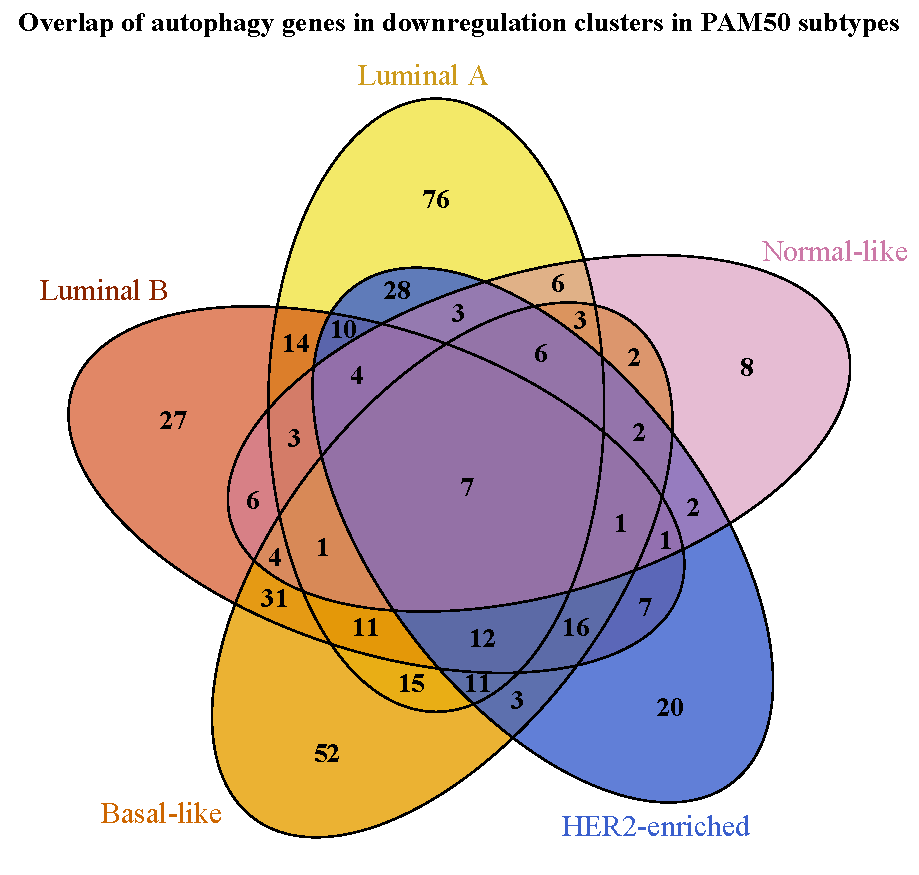
\includegraphics[scale=0.5]{overlap_clusters.pdf} 
            \caption[Overlap between PAM50 subtype-specific downregulation cluster autophagy genes]{Venn diagram showing overlap between PAM50 subtype-specific autophagy genes assigned to downregulation clusters in clustering of individual subtypes.}
            \label{fig:overlapclusters}
            \end{figure}
            
Remarkably, each subtype has a fairly large number of  genes unique to its downregulation cluster, e.g. Luminal A -- 76 genes. There is a very low number of genes that are downregulated in all subtypes -- 7 genes; or 19 (7+12) genes, if not taking into account Normal-like clustering data, as it may be affected by only having three stages. Luminal A and B share 62 genes, Luminal A and Basal-like - 67 genes , and Luminal A and Basal-like -- 83, but between three of them, only 11 genes. This suggests that, overall, different subsets of autophagy genes are downregulated in different PAM50 subtypes. 



            

In differential expression analysis, one of the tested models (Group1: PAM50+stage) allowed the comparison of each individual stage of every subtype to normal samples. In this way, downregulated autophagy genes at each stage in every subtype were identified. Table \ref{table:autodown} show the numbers of differentially expressed genes autophagy in each subgroup combination (vs normal). 

    %TABLE autophagy downreg
\begin{table}[!h]
\centering
\tiny
\caption[Count of differentially expressed autophagy genes in contrasts with normal samples]{Count of differentially expressed autophagy genes detected in contrast of Group1 model. Gene counts for each stage of each PAM50 subtype when compared to normal are shown.  }
\label{table:autodown}
\begin{tabular}{l|c|c}
\multicolumn{1}{c|}{\textit{DE contrast (vs normal)}} & \begin{tabular}[c]{@{}c@{}}upregulated\\  genes\end{tabular} & \begin{tabular}[c]{@{}c@{}}downregulated\\  genes\end{tabular} \\ \hline
\multicolumn{1}{|l|}{Luminal A, stage 1} & 65 & \multicolumn{1}{c|}{122} \\ \hline
\multicolumn{1}{|l|}{Luminal A, stage 2} & 64 & \multicolumn{1}{c|}{127} \\ \hline
\multicolumn{1}{|l|}{Luminal A, stage 3} & 56 & \multicolumn{1}{c|}{116} \\ \hline
\multicolumn{1}{|l|}{Luminal A, stage 4} & 30 & \multicolumn{1}{c|}{59} \\ \hline\hline
\multicolumn{1}{|l|}{Luminal B, stage 1} & 65 & \multicolumn{1}{c|}{147} \\ \hline
\multicolumn{1}{|l|}{Luminal B, stage 2} & 77 & \multicolumn{1}{c|}{156} \\ \hline
\multicolumn{1}{|l|}{Luminal B, stage 3} & 86 & \multicolumn{1}{c|}{154} \\ \hline
\multicolumn{1}{|l|}{Luminal B, stage 4} & 74 & \multicolumn{1}{c|}{136} \\ \hline\hline
\multicolumn{1}{|l|}{Basal-like, stage 1} & 81 & \multicolumn{1}{c|}{152} \\ \hline
\multicolumn{1}{|l|}{Basal-like, stage 2} & 83 & \multicolumn{1}{c|}{182} \\ \hline
\multicolumn{1}{|l|}{Basal-like, stage 3} & 72 & \multicolumn{1}{c|}{173} \\ \hline
\multicolumn{1}{|l|}{Basal-like, stage 4} & 59 & \multicolumn{1}{c|}{141} \\ \hline\hline
\multicolumn{1}{|l|}{HER2-enr., stage 1} & 75 & \multicolumn{1}{c|}{155} \\ \hline
\multicolumn{1}{|l|}{HER2-enr., stage 2} & 74 & \multicolumn{1}{c|}{182} \\ \hline
\multicolumn{1}{|l|}{HER2-enr., stage 3} & 82 & \multicolumn{1}{c|}{173} \\ \hline
\multicolumn{1}{|l|}{HER2-enr., stage 4} & 43 & \multicolumn{1}{c|}{141} \\ \hline\hline
\multicolumn{1}{|l|}{Normal-like, stage 1} & 28 & \multicolumn{1}{c|}{49} \\ \hline
\multicolumn{1}{|l|}{Normal-like, stage 2} & 37 & \multicolumn{1}{c|}{48} \\ \hline
\multicolumn{1}{|l|}{Normal-like, stage 3} & 19 & \multicolumn{1}{c|}{22} \\ \hline
\end{tabular}
\end{table}

\newpage


\begin{wrapfigure}{R}{0.4\textwidth}
        \hfill
        \captionsetup{justification=centering}
        \centerline{ 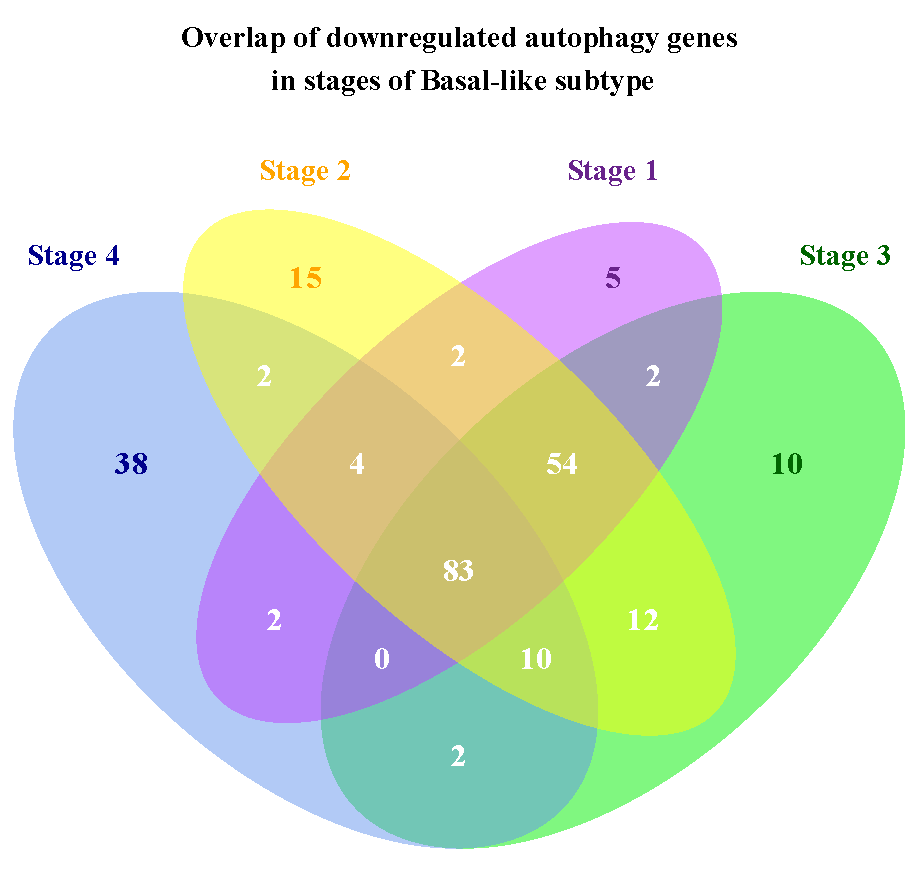
\includegraphics[width=0.38\textwidth]{venn_basal.pdf}}
        \label{fig:vennbasal}
        \vspace*{-8mm}
        \caption[Overlap between downregulated autophagy genes in stages of Basal-like subtype]{Overlap between downregulated autophagy genes \\in stages of Basal-like subtype}
        \end{wrapfigure}
 

By overlapping the these genes, it is possible to get an insight into which genes are downregulated at in all stages of one subtype, and also which and how many genes are specific to a particular stage. 

Figure \ref{fig:vennbasal} shows such overlap for Basal-like subtype. There are 83 autophagy genes that are downregulated in all stages. 54 genes are downregulated in stages 1-3 but not in stage 4. Also, stage 4 has quite a lot of genes (38) downregulated specifically in it.\\
Figure \ref{fig:vennluma} shows the stages overlap for Luminal A. Again, as for Basal-like, the two largest overlap group are between all stages (54 genes) and between stages 1-3 only (57 genes). Interestingly, in stage 4 of Luminal A there are not that many unique genes as in Basal-like.\\

\begin{wrapfigure}{L}{0.45\textwidth}
        \hfill
        \captionsetup{justification=centering}
        \centerline{ 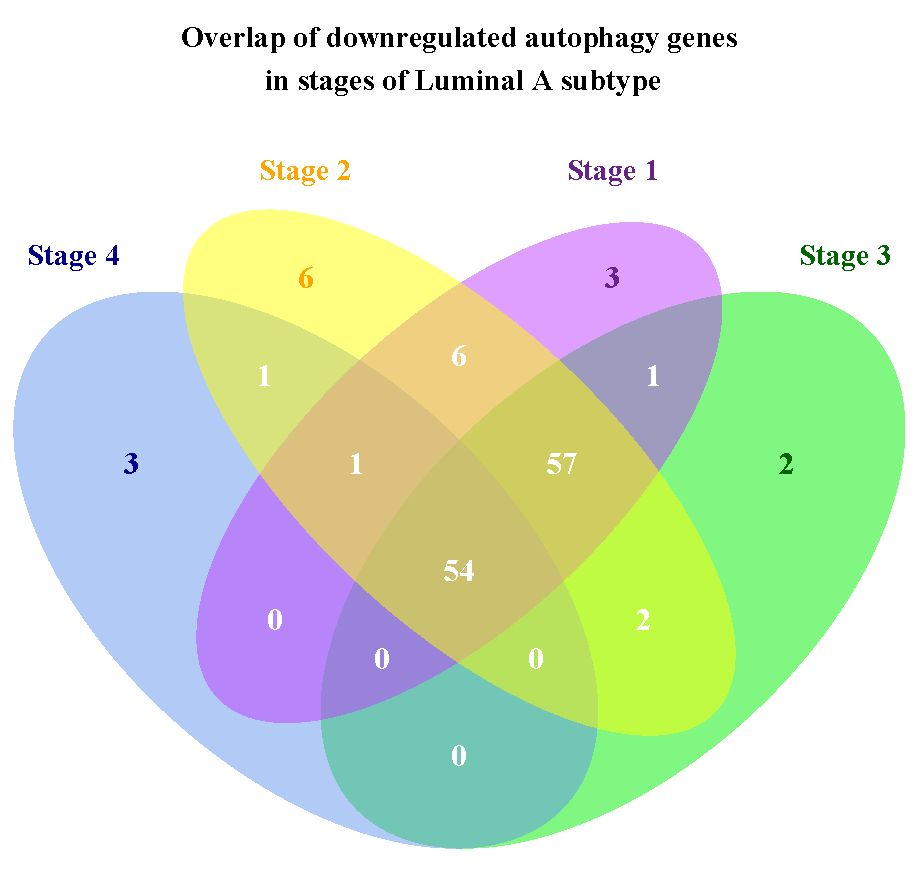
\includegraphics[width=0.38\textwidth]{venn_lumA.pdf}}
        \label{fig:vennluma}
        \vspace*{-8mm}
        \caption[Overlap between downregulated autophagy genes in stages of Luminal A subtype]{Overlap between downregulated autophagy genes \\in stages of Luminal A subtype}
        \end{wrapfigure}
       

%\vspace{5mm} 
The analogous Venn diagrams for Luminal B, HER2-enriched and Normal-like subtypes are available from Appendix X4.

In Luminal B there are 87 genes shared by all stages, 40 genes shared by stages 1-3, and 31 genes unique to stage 4, showing a similar scenario to Basal-like. In HER2-enriched, the largest overlap group is stages 1-3 (79 genes), whereas all stages share only 32 genes. Normal-like subtype is a slightly different case, as there are not stage 4 samples, and in addition to it inherent similarity to normal samples, which resulted in fewer DEGs in total. In normal like, there are only 12 samples shared by the available stages (1-3). 



